\documentclass[12pt, a4paper, oneside]{article} % Paper size, default font size and one-sided paper
%\usepackage[dcucite]{harvard}
\usepackage{tikz}
\usetikzlibrary{shapes, shadows, arrows}
\usepackage{rotating}
\usepackage{amsmath}
%\usepackage{setspace}
\usepackage{pdflscape}
\usepackage[flushleft]{threeparttable}
\usepackage{multirow}
\usepackage[comma, sort&compress]{natbib}% Use the natbib reference package - read up on this to edit the reference style; if you want text (e.g. Smith et al., 2012) for the in-text references (instead of numbers), remove 'numbers' 
\usepackage{graphicx}
\graphicspath{{./Figures/}} % Specifies the directory where pictures are stored
%\bibliographystyle{plainnat}
\usepackage{listings}
\bibliographystyle{agsm}
\usepackage[colorlinks = true, citecolor = blue, linkcolor = blue]{hyperref}
%\hypersetup{urlcolor=blue, colorlinks=true} % Colors hyperlinks in blue - change to black if annoying
\begin{document}
%\renewcommand[\harvardurl]{URL: \url}
\title{Carry trade and transmission}
\author{Rob Hayward\footnote{University of Brighton Business School, Lewes Road, Brighton, BN2 4AT; Telephone 01273 642586.  rh49@brighton.ac.uk} and  Jens H\"{o}lscher\footnote{Professor of Economics, Bournemouth Business School, Bournemouth University, jholscher@bournemouth.ac.uk, Tel: 01202 965392.}} 
\date{\today}
\maketitle
\begin{abstract}
The level of international risk aversion is shown to affect the probability of financial crash in a range of European countries.  The evolution of financial stability is assessed by looking at carry-trade  returns.  These returns may be drawn from one, two or three financial regimes.  The two-regime model is the best fit for most countries.  The proability of switching from a regime of financial \emph{calm} to a financial \emph{crash} is affected by the level of the risk aversion.   
\end{abstract}

\section{Introduction}
As the size of international capital flow has increased in absolute terms and relative to expansion of the trade in goods and services it has also become subject to less regulatory constraint. Economic authorities have faced repeated struggles with financial instability that has an international source.  An inflow of capital from abroad can appear superficially attractive but its arrival can cause goods and asset price inflation, it can shape institutions, economic development and political opinion, and, most importantly, the portfolio flows can disappear even more swiftly than they arrive.  %Transition and emerging economies have been particularly affected by international financial crises.  %The financial systems of transition and emerging economies are less developed than those of the the international finance centres and therefore there is scope in these countries for the financial sector to increase in size and relative to overall level of economic activity.  This process can attract financial entities from more developed economies. \citet{ONBcarry} and \citet{EBRD} survey the expansion of Euro area banks into the Central and Eastern European trasition economies; \citet{Gabor} discusses the political economy of this \emph{financialization} where the financial system expands to new sections of the economy.  

%Bernanke speaking to Joint Economic Committee on 22-May-13.  Speaking about moderating asset purchase, but not yet. 
%http://www.federalreserve.gov/newsevents/testimony/bernanke20130522a.htm

International financial conditions following the 2007-08 crisis have fuelled the growth of investments in transition and emerging economies by providing large amount of funding-currency liquidity in the financial systems of developed economies at the same time as those countries that were ourtside the immediate financial crisis have offered relatively attractive investment opportunities.   The negative May 22nd 2013 market reaction to indications from US Fed Chairman Bernanke that US monetary policy could be tightened has drawn attention to the risk of financial crisis caused by capital outflows and has encouraged some reassessment of the relationship between capital flows and international monetary policy, international liquidity and international risk aversion.  

\citet{Cerutti2014} ask three questions:  what drives global liquidity; where does the global liquidity cycle originate; and, how can the borrowing country manage its exposure to global liquidity? Their focus is on cross-border banking flows. They find that global liquidity is affected by uncertainty and risk aversion and that uncertainty and risk-aversion are highly correlated across countries. However, their research shows that bank conditions and monetary policy actions in countries outside the US can also exert influence. They have three specific findings:  cross-border bank-lending falls when international risk aversion increases, when US dealer bank leverage falls or there is an increase in term premia; there is a small interest rate effect on capital flows; US and European domestic credit conditions and monetary policy affect lending to other regimes, US monetary policy is important and European leverage and credit conditions are important.  They conclude that while the US drives the global liquidity cycle through its monetary policy, other financial centres (particularly European) affect the financial cycle through the conditions of their banks. Their work suggests that global liquidity is affected by global financial conditions rather than monetary policy.

%\href{http://www.federalreserve.gov/pubs/feds/2014/201446/201446abs.html}{Fed Paper} 
Flight-to-Safety (FTS) is the term used to describe the sharp move of capital towards international financial centres and relatively safe assets.\citet{FTS} find that FTS are relatively rare events. Their study of of 23 countries finds that FTS represent less than 3\% of the sample of daily data that runs from January 1980 to January 2012.  In a contrast to other work, they find that most of the events are country specific (they characterise on 25\% as "global") and are associated with an increase in the VIX index and the TED spread.\footnote{The VIX is an index of implied volatility on options from the S\&P 500 index.  It is commonly used as a measure of international risk aversion as it signals increased demand by fund managers for option protection.  See \citet{VIX}, \citet{GoldmanVol} and \citet{Diamond} for fuller details.The TED spread is the spread between the treasury bill and the Euro-dollar rate.  It is used as a market measure of perceived credit risk of financial institutions as it records the risk premium that investors require to lend to banks relative to the risk-free rate.}   %These FTS eposodes are also associated with lower levels of consumer sentiment, appreciation of the  Yen, Swiss franc and US dollar funding currencies. %Financial, basic materials and industrial industries under-perform in FTS periods while telecoms outperform; money market instruments, corproate bonds and commodity prices (other than precious metals) face abnormal negative returns, hedge funds (particularly "event-driven" display negative FTS beta.  Liquidity deteriorates on FTS days in bond and equity markets. Economic growth and inflation decline in the year after a FTS event. 

%\href{http://www.imf.org/external/pubs/cat/longres.aspx?sk=41655.0}{IMF:  Impact of Fed tapering annoncement on emerging markets}.  

Consistent with the evidence of an interplay between monetary policy and international risk, and between domestic and international factors, \citet{Ahmed2014} find that economic growth, interest rate differentials and the level of global risk appetite are all important determinants of private capital flows to emerging markets.  They also suggest that capital flows have been more sensitive to interest rate differentials since the financial crisis of 2007-08. There is also some evidence here that quantitative easing has had some effect on capital flows. 

\citet{IMFLatam} use a panel VAR method to assess the effect of US monetary policy since 1990 on capital flows to 38 emerging economies, finding evidence that Fed tapering while not necessarily leading to capital outflow, could generate \emph{new risk premium shocks}.   If investors require a higher return, asset price falls are required. 

While the origin of international financial crisis may be international, US monetary policy for example, the effects may vary by asset class and, US policy can influence different countries in a variety of ways.  Using daily data on exchange rates, stock prices and emerging market bonds, \citet{Tapering} find that exchange rates and bonds are less affected by international liquidity shocks than stock markets.  They also find that stronger domestic macroeconomic fundamentals, more prudent financial policy and deeper financial markets provide some insulation against US monetary policy shocks.

One specific part of the range of international capital flows that has attracted particular attention because it is associated with speculation is the \emph{carry-trade}.  This is the attempt to take advantage of the break down in \emph{uncovered interest parity} (UIP)\footnote{See xxx for an overview of the breakdown in UIP and .... for more on the carry trade} by funding an investment in relatively high yielding transition currencies with a low interest base.  UIP is the theory that interest rate differentials between currencies should be matched by an equal expectation that the low rate currency will appreciate against the higher rate until expected returns from the activity are reduced to just a compensation for taking risk. %The base currencies are the US dollar, the Euro, the Swiss franc and the Japanese yen.  These are the safe-haven currencies used in \citet{HabibStracca}, and they are base units that are found to appreciate during periods of FTS in \citet{FTS}. 

There is widespread evidence that UIP does not hold on average (see \citet{FrootAnomolies}. \citet{FrootFrankelFDB}, \citet{Hodrick1987} and \citet{SpronkEER} for some of the discussion) but this does not guarantee that excess returns are possible.  These returns disappear when a more multifaceted assessment of risk is applied.  The small risk of a large loss, is either something that many investors wish to taoid by paying to transfer the risk to other entities.  It is also a risk that is often ignored or misperceived by myopic, over-confident economic agents suffering behavioural biases. Carry-trade returns are compensation for taking \emph{crash-risk}.  

\citet{BrunnermeierCarry} analyses a sample of carry trades and find that the returns are characterised by negative skew and a larger than normal risk of extreme loss; \citet{JurekCrash} assesses the cost of purchasing option protection against crash-risk and finds that it covers a proportion of the excess returns that seem to be generated by the carry-trade; \citet{Hayward2013} compares carry returns in period of calm and periods of crisis (as measured by elevated levels of the VIX index) and finds that carry returns a negative, skewed and fat-tailed when international risk aversion is heightened, but a more normal, positive return when conditions are calm. 

 
\citet{NYFedtaper} consider the effect of changes in global risk aversion on the carry-trade.  They find that the initial signal from the US central bank in Fed Chairman Bernanke's May 22 2013 testimony to Congress coincide with an increase in global risk aversion which affected global asset prices. %They use the approach presented by \citet{MertensSVAR} to estimate the effect of policy changes by using a two-stage least squares appraoch to identify the SVAR model of asset price changes.  
By identifying the performance of exchange rates without a change in risk aversion, they suggest that nearly half of the depreciation of a basket of 45 carry-trade currencies with the largest one-month interest rate relative to a basket of the US dollar and other equally low rate currencies is explained by this increased risk aversion. They find that nearly all the decline in Emerging market equities is attributable to the increase in risk aversion.

There is evidence that the international financial cycle is increasingly global \citet{Rey2013}, \citet{Obstfeld2014} and \citet{Bruno2014}.  %\href{http://www.voxeu.org/article/primer-global-liquidity}{VOX: GLobal Financial Liquidity}. 
For example, there is evidence the correlation of cross-border credit growth has increased since the 1990s and that, funds increasingly flow from the financial centres to the rest of the world. As such \citet{Cerutti2014} find that credit and liquidity contractions in  the US, Euro zone, UK and Japan affect the rest of the world. Credit supply in financial centre economies affect the provision of cross-border credit.  This is what they call \emph{global funding liquidity}, a feature that affects financial conditions globally. 

%The theme of this recent research is of an interplay between international and domestic factors.  It is clear that there are a range of features, including economic, institutional and cultural that can affect this interation and the evolution of interaction of international financial risk. 


%Do the next two paragraphs set up the dicotomy between the domestic factors and the international (flight-to-quality) factors?  THere are a range of facts:  EM debt rose from 650bn in 2001 to 6.9tn in 2013 according to BIS data.  

%\subsection{The instability cycle}
%The aim of this study is to understand more about the evolution of internatonal financial instability by studying the carry trade in a number of European transition and emerging economies. There are two related areas of interest:  the factors that trigger a crash, reversal or sudden-stop; the way that the financial system evolves to the point where the crash is likely to take place.  There have been a number of attempts to identify levels of finacial risk.  This has clearly become even more of an issue since the financial crisis.  For example, \citet{IFCMeasure}.  The IMF have developed a range of \emph{Financial Soundness Indications} (IMF 2006).     Also - Hawkins and Klau (2000), Nelson and Perli (2005) and Gray et al (2007).  There are six main strands:  the real sector, including fiscal position and inflation; the corporate sector, specifically the level of debt and overseas exposure; the ability of the household sector to weather downturns; the external sector, including the foreign exchange position and the capital account; the financial sector; finacial markets. 

%A number of studies applied the early warning indicator methods initially developed in the literature for currency and balance of payments crises to banking crises. Earlier work includes, among others, Calvo et al (1993), Eichengreen et al (1996), Turner and Goldstein (1996) Frankel and Rose (1996). Demirgüç-Kunt and Detragiache (1997) use a multivariate Logit approach to identify determinants of banking crises in a large panel of developing and industrialised countries: slow GDP growth and high inflation, vulnerability to sudden capital outflows, low liquidity in the banking sector, a high share of credit to the private sector, past credit growth, explicit deposit insurance and weak institutions. Kaminsky and Reinhardt (1999) identify early warning indicators of twin (banking and balance of payments) crises, such as credit and equity prices, by looking at the ability of such variables to predict crises 12 or 24 months a, while minimising the noise3  to signal ratio. Borio and Lowe (2002) and Borio and Drehmann (2009) build on the techniques developed by Kaminsky and Reinhardt (1999). Like the latter, they define threshold values for the indicators, but unlike them, they look at cumulative processes rather than just growth rates over one year, they use ex ante information (ie information which was available to the policymaker prior to the crisis) and, for the first time, they consider combinations of indicators and look at multiple time horizons. BIS Goodhart 2006%

%However, While measuring debt-to-equity ratios and the scale of bank lending may provide some indication about the regime that is in place, this is imprecise and it is clear that financial services business evolve in ways that make loan counting  inadequate.The recent financial crisis showed that innovations like \emph{Collateralised Debt Obligations (CDO)} can allow an increase in debt that does not directly in bank lending. 

%Does this go first?
\subsection{The evolution of financial instability}
International financial risk and the carry-trade are beset by \emph{peso problems}. Peso problems are cases where there is  potential for discrete shifts in the distribution of variables.  This can affect expectations, risk-premia and asset pricing models. In \citet{evans199621}, for example, if $s_t$ is the log of US dollars in terms of Mexican peso and the peso is fixed at 0.08 dollars and this is state $s^0$ with a expected probability at time $t$ of $\pi_t$ that there will be an exchange rate adjustment to $s^1$, the expected depreciation is 
\begin{equation}
E[s_{t+1}|\Omega_t] = \pi_ts^1 + (1 - \pi_t)s^0
\end{equation}
Therefore, the difference between the realised and expected rate is 
\begin{equation}
s^0 - E[s_{t+1}|\Omega_t] = \pi_t(s^0 - s^1)
\end{equation}

%A common problem in estimating economic models is that the parameters do not tend to be stable over time.  A HMM can be used to model a range of cases that can span a simple transition from one state to another, switching between multiple regimes with varying parameters towards the extreme where the number of regimes mean that system is close to having time-varying parameters (TVP).  

Expectations are continually confounded though they are not formed in an irrational way. In these cases, modeling the two regimes and the probability of switching between the two would would improve understanding.  It is also useful in allowing non-linear relationships between variables and for incorporating a range of cases that can span a simple transision from one state to another to an extreme of multiple states where parameters are close to time-varying.  \citet{hamilton1988rational} used a Hidden Markov Model (HMM) to incorporate discrete changes in expectations about Fed policy to make a closer match between the expectations theory and the term structure of interest rates data.  This technique assumes that unobserved regimes will switch from one state to another with a given probability.  \citet{Hamilton1989} also analysed the performance of postwar US GNP with adjustments from periods of positive to negative growth. The regime shift is modelled as a first-order Markov process.  In other words, state $S_t$ depends only on the previous state $S_{t-1}$, and these are given probabilities that the state will switch or remain unchanged.  The parameters of an ARIMA representation of US GNP shift between the two regimes so that there is a 3\% decline in the US growth rate during a recession.  
%\emph{The peso problem} describes a range of cases where there is a large, descrete shift or \emph{jump} in the system.  This is particularly relevant to the carry-trade as one explanation for the evidence of a breakdown in UIP is that exchange rate expectations cannot be modeled by taking the average of past realisations. 


%The raw model just assume that there are three states with random allocation of the starting values.  However, the initial estimates of the regime parameters can come from the estimates made in the doctorate using the crash and caution identification from the VIX; the initial estimates of the priobabilities of each state can come from the percentage of each state in the final version of the model that is run without initial estimates.  

%I think that $\theta_1$ on page 4 of the depmixS4 vignette is the parameter that nees to be set. 

%At the top of page 10 of the vignette, there is an example of how the transition matrix may be augmented by a model.  I do not understand this fuilly, but it may be possible to link the transition to the VIX index.  Obviously, there is some risk of circularity here. Anyway, it may be useful to compare the difference. 


\citet{schaller1997regime} extend the Hamilton model to assess stock returns in two regimes, uncovering strong evidence of regime-switching in the mean and variance of US stock returns.  They also find that that the response of stock returns to the price-dividend ratio is asymmetric; \citet{dueker1997markov} analyses the change in stock market volatility that arise from different regimes. Markov models switching models are also typically used to understand the evolution of credit risk.  A firm with a particular credit rating has a given probability of maintaining that rating or moving to another.  This can be used to estimate probability of default and value corporate bonds (reference needed).  \citet{frydman2008credit} use a mixture model against the alternative of a pure Markov chain. The observed rating changes relate to two different underlying Markov chains representing the evolution of credit ratings.  There is a heterogeneity that seems to depend upon the industry.  For example, ratings of firms in the retail and wholesale trade sectors tend to be more dynamic than the others. 

%Agn Timmerman (2011)
%Looking at how abrupt changes in regime can lead to changes in the way that the system works.  The different regimes can be associated with different underlying distribution of returns.  This can allow the understanding of the non-liner and non--normal distribution within  normal or linear framework.  At the extreme, the regime switch model can incorporate a \emph{jump model} with one change, and can also be associated with time-varying parameter models that have a large number of regimes.

%The broad framework for the method is to model a discrete state $s_t \in %\{0,1,\dots k \}$
%\begin{equation}
%y_t = \mu_{s_t} + \phi_{s_t} y_{t-1} + \sigma_{s_t} \varepsilon_t, \quad %\varepsilon_t \sim iid(0,1) 
%\end{equation}

%The process governing the underlying regime must also be defined. 

%\begin{equation}
%Pr(s_t = 0| s_{t-1} = 0) = p_{00} \quad \text{and} \quad Pr(s_t = 1| s_{t%-1} = 1) = p_{11}
%\end{equation}

%More generally, the transition could be time-varying and could be dependent on the time spent in the regime.  See Durland and McCurdy (1994) for example of the probbilities  in the transition matrix being related to time. The longer the systemm has remained in the build phase, the greater the risk of crash.  Remember that the crash phase is a period when there is risk of a sharp reversal.  

%See Diebold, Lee and Weinbch (1994) for examples where the transition probabilities depend on some other state variables.  For example, the interest rate spread.   Could the VIX index or other factors be used?  Vix index would indicate heightened international tension as one element that affects the probability of transforming from one state to the next.  An elevated VIX is an indication of the heightened international risk premium.  This may increase the probability that the regime switches from carry build to crash.  This is a theme that could be related to the bubble bursting so any information that improves the ability to identify bubbles bursting would be beneficial.  


%There are two states of the world:  crisis and moderation.  If the system is in a crisis, it stays there with probability p; it switches to moderation with probability $1-p$.  If in moderation, the system stays there with a probability q and switches to crisis with probability $1-q$.  If the probabilities change over time, there is no longer a \emph{homogenous Markov Chain}. Ghysels has a seasonal dummy for the probabilities that represent the months or quarters.  

%Can the probabilities change over time?  This may be the result of changes in the resilience of the financial system. 
%\href{http://members.home.nl/jeroenvermunt/dias2010.pdf}{Mixture Hidden Markov Models} Hidden models help to calafify the regime under which securities trade. Model takes into account the unobserved hetrogeneity across time. This could could be extended to space (for different countries).  Is it possible to estimate a panel? 

%Can the systemm be used to compare to fixed and floating exchange rates. 

%The use of the regime-switch allows the transition from one regime to another to be the result of something that is more than just a deterministic process. There are a number of ways that this model could be expanded.  Dueker has a model where the degrees of freedom from a Student-t distribution change with the regime.  

%An alternative way to look at this would be to use a TAR mode.  

%There are three main ways that the evolution of international financial risk can be modelled.  The first is through a one-off transition from calm to crisis. This represents a world there has been some major event that has transformed the system and where there has been a permanent adjustment from one regime to another.  This is a one-off switch that may be a function of political or policy changes that are permanent. For example, this could be caused by a move from a fixed exchange rate to something more variable or another type of shift in monetary policy regime.   

%The second and moris a two-regime model where there is a switch between periods of calm and crisis.  This is  a relatively simple system where the interest is in the factors that can trigger an adjustment from one regime to another.  A more sophisticated version of this is the third model were there is an evolution of the system from a position of calm, through a time when speculative positions are build and then into a crash. 

%The third is a more sophistocated model that would add further dynamics. 

%The relatively simple model that switches between periods of calm and crisis has been discussed by \citet{DornbuschSS}, \citet{CalvoSS} and \citet{KrugmanSS}.  The term \emph{sudden stop} emphasises the importance of the inflow of international capital that takes place before the disruptive effects of reversal.  

%other references 
 %Abiad, A., 2003. Early-Warning Systems: A Survey and and a Regime-Switching Approach. IMF Working Paper No.03/32. International Monetary Fund.
 %Aziz, J., Caramazza, F., Salgado, R., 2000. Currency Crises: In Search of Common Elements. IMF Working Paper No.00/67. International Monetary Fund
 %Calvo, G., 2000. Balance-of-Payments Crises in Emerging Markets: Large Capital Inflows and Sovereign Governments, in: Krugman, P. (Ed.), Currency Crises, University of Chicago Press, Chicago, Illinois,
% \href{http://mpra.ub.uni-muenchen.de/383/}{http://mpra.ub.uni-muenchen.de/383/}

%Minsky's \emph{Financial Instability Hypothesis} (FIH) presents a model of endogenous financial crisis where a period of economic calm creates the conditions for more adventurous and risky financial behaviour that increases the fragility of the system \citet{MinskyStabilising, MinskyKeynes, MinskyFIH, MinskyLongerWaves}.  Minsky identified three phases of financing:  hedge, speculative and Ponzie.  

%In the first of these the system is stable as lending is not excessive, borrowers are cautious and revenues are generally sufficient to ensure that repayments of principal and interest can be made from current income.  This period may be framed by memories of past financial crisis and the economic hardships that are associated with it.  Violent economic shocks are among the range of possible outcomes that can readily be envisaged by creditors and debtors, encouraging them to be cautious and risk-averse. 

%However, in the absence of economic shocks these memories of hardship fade further into the background and all parts of the economic and financial system become more prepared to take risks.  Lending becomes more speculative; decision-making gives less weight to the possibility of extreme outcomes and put more emphasis on the immediate experience of economic calm.  The increase in lending tends to improve immediate economic conditions:  business investment and consumer spending rise if lending is broad-based; asset prices will appreciate where lending is directed towards financial investment.  The increase in economic activity that comes from this expansion in credit will feedback to improve immediate economic conditions, exacerbating the sense of well-being and undermining the arguments of those preaching more cautious behaviour.  Positive feedback effects cause a non-linear relationship between credit growth and economic activity and between credit and asset prices. 

%\citet{BernankeGertler}, \citet{Bernanke1999chapter} and \citet{Azaraidis} present models where there is a non-linear relationship between  the provision of credit and the level of economic activity. \citet{BernankeGertlerAgency} show how balance sheet dynamics can affect the business cycle through a reduction in the agency cost of business investments and \citet{Balke} has a non-linear model of credit shocks.  \citet{Avdjiev2014} use a three regime Threshold-Vector-Auto regression (TVAR) to identify the non-linearities in credit market shocks.  They find that credit shocks have the greatest impact when output growth is above its long-term trend. 

%While credit becomes more plentiful, household and business managers become more optimistic.  There is evidence that decision-making tends to favour outcomes that are more recent, apparent or those that that can be more easily envisaged (see for example, \citet{KTAvailability} and \citet{Schwartzavailability} for some evidence on the \emph{availability heuristic} and related literature).   % more required or footnote? 

%In this way, the repayment of loans becomes increasingly dependent on the continuation of above-normal economic conditions or the appreciation of asset prices.  If this process is allowed to continue, a speculative frenzy can take hold.  Economic agents are dragged into the euphoria as households compete with the conspicuous consumption of their neighbours, businesses investment expands to increase capacity and market share in the face of booming demand, while property and financial market speculators redouble their bets.  \citet{BrunnermeierLiquidity} show how the link between the availability of credit for investors and the level of liquidity in financial markets can create \emph{liquidity spirals}.   They note that the capital of speculators can drive market liquidity, risk premia and asset prices.  The ability to be able to borrow against collateral is particularly important here.  As asset prices increase, the ability to borrow against their value raises the amount of trading credit that is available.  

%The conditions are now in place for the bubble to burst in a violent reversal.  \citet{FisherBD, FisherDD} explained the way that \emph{debt-deflation} could create a ricochet between the financial and real sectors of the economy with a decline in the availability of credit exacerbating the financial strain on households and business, helping to reduce household and business spending thereby raising the quantity of bad loans and the sense of caution at financial institutions. In financial markets, credit and liquidity disappear and the decline in asset value affects the ability of institutions to raise funds.  Fire sales in illiquid markets exaggerate the fall in prices. \citet{ReinhartRogoff} reveal how credit booms help to explain the breadth and depth of post-boom recessions.  The catalyst for the collapse is difficult to pin down as the build up to the excess is fragile.  See \citet{Gorton2013} and \citet{BrunnermeierLiquidity} again for financial market effects. The economic consequences are profound.  

\section{A Markov model of financial stability}
Financial stability for each of the countries covered is presented as a first-order Markov process.  There are three possible cases:  a single regime that does not change; a two-regime model that switches from calm to crisis with a sub-model that makes a one-off switch and does not return; and, a three-regime model that will switch from calm, through the building of risky investments before moving to the crash.  

The base model with one regime is a control that assess whether regime-switch is appropriate.  The one-off switch could represent a single change in political or economic policy that contributes to a step change in financial conditions.  It is more likely that there will be a propensity to switch between periods of calm and crisis has been discussed by \citet{DornbuschSS}, \citet{CalvoSS} and \citet{KrugmanSS}.  The term \emph{sudden stop} emphasises the importance of the inflow of international capital that takes place before the disruptive effects of reversal.  A three regime model could represent an evolution of financial instabilty along the lines of \citet{MinskyKeynes, MinskyFIH, MinskyLongerWaves} where conditions of financial calm encourage excess lending and an accumulation of financial risk before a crash.  This could be an evolution of caution, building and crash.  

In situations like this where the underlying financial regimes are not observable, the Markov model is not sufficient to fully describe the process. It may nonetheless be possible to identify a probabilistic relationship between the carry-trade returns and the underlying financial regime and to use this to uncover the parameters of a \emph{Hidden Markov Model (HMM)}. 
 
\subsection{The HMM model}
Figure \ref{figref:HMM2} gives an overview of the system.  The HMM has three components: $\pi, A, B)$ where,

\begin{itemize}
\item The prior model: $P(S_n|y, \theta_{prior})$ $(\pi)$
\item The transition model: $P(S_t|y, S_{t-1}, \theta_{trans})$ $(A)$
\item The response model: $P(Y_t| S_t, y, \theta_{resp})$ $(B)$
\end{itemize}

Where $S_n$ are the $n$ states or regimes; $y_t$ are the observed carry-trades; and $\theta_{prior}$, $\theta_{trans}$ and  $\theta_{resp}$ are the parameters of the prior, transition and response models respectively. The unobserved financial regimes are modelled as a Markov chain that switches from a period of calm to crisis.  The returns to the carry-trade are more likely to take particular characteristics according to the underlying regime.   


\begin{figure}
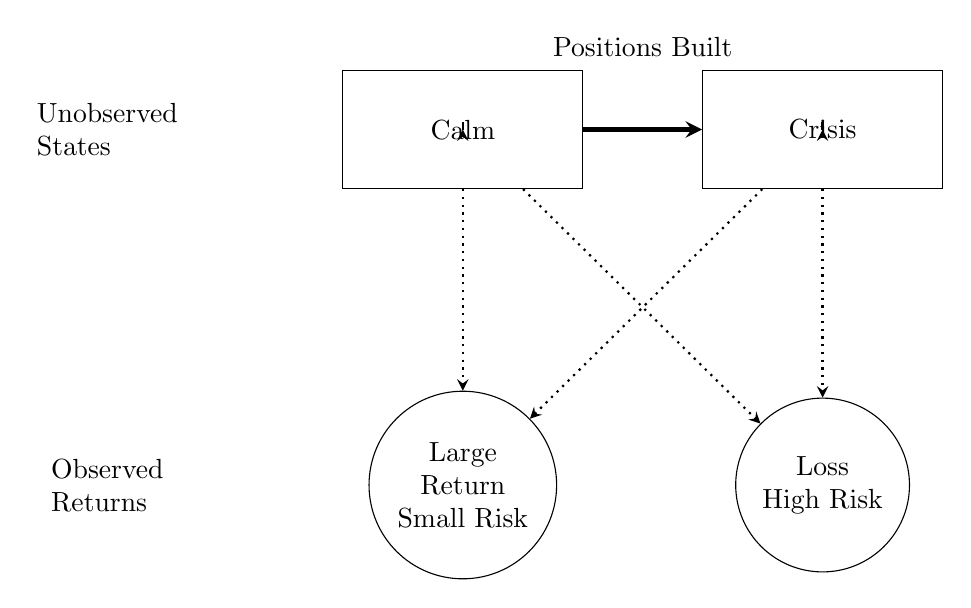
\begin{tikzpicture}
\tikzstyle{decision} = [circle, draw, minimum height = 8mm, 
  text width = 5em, text centered];
\tikzstyle{line} = [draw, -stealth, thick]
\tikzstyle{line2} = [draw, -stealth, ultra thick]
\tikzstyle{line3} = [draw, -stealth, dashed, thick]
\tikzstyle{line4} = [draw, -stealth, dotted, thick]
%\tikzstyle{elli} = [draw, ellipse, fill = red!50, minimum height = 8mm, 
 % text width = 5em, text centered]
\tikzstyle{block} = [draw, rectangle, text width = 8em, 
  text centered, minimum height = 15mm, node distance = 8em]
\node [block](Calm){Calm};
%\node [block, left of  = Build, xshift = -5em] (Calm){Calm}; 
\node [block, right  of = Calm, xshift =5em] (Crisis){Crisis};
\node [decision, below of = Calm, yshift = -10em, align = center]
(Calm2) {Large Return \\ Small Risk}; 
\node [decision, below of = Crisis, yshift = -10em](Crisis2) {Loss \\ High Risk};
%\node [decision, below of = Caution, yshift = -10em, align = center](Caution2) 
%{Small \\ Return \\ Average \\ Risk};
%arrows 
\path [line3] (Calm) -- (Calm);
\path [line3] (Crisis) -- (Crisis);
%\path [line3] (Crash) -- (Crash2);
\path [line2] (Calm) -- node [yshift = 3em] {Positions Built} (Crisis);
%\path [line2] (Caution) -- node [yshift = 3em]  {Speculative Lending} (Build);
\path [line4] (Calm) -- (Crisis2);
\path [line4] (Crisis) -- (Calm2);
\path [line4] (Calm) -- (Calm2);
\path [line4] (Crisis) -- (Crisis2);
%\path [line4] (Crash) -- (Caution2);
%\path [line4] (Crash) -- (Build2);
\node [align = left, left of = Calm, xshift = -10em] {Unobserved \\ States};
\node [align = left, left of = Calm2, xshift = -10em] {Observed \\ Returns};
%\path [line] (decision1) -| node [yshift = 0.5em, 
%   xshift = 8em] {YES} (process 1);
%\path [line3] (Crash) -- (Caution); 
% 	xshift = -8em] {NO} (process 2);
\end{tikzpicture}
\caption{Two-Regime Hidden Markov Model (HMM)}
\label{figref:HMM2}
\end{figure}




%\begin{landscape}
%\begin{figure}
%\begin{tikzpicture}
%\tikzstyle{decision} = [circle, draw, fill = yellow!30, minimum height = 8mm, 
%  text width = 5em, text centered];
%\tikzstyle{line} = [draw, -stealth, thick]
%\tikzstyle{line2} = [draw, -stealth, ultra thick]
%\tikzstyle{line3} = [draw, -stealth, dashed, thick]
%\tikzstyle{line4} = [draw, -stealth, dotted, thick]
%\tikzstyle{elli} = [draw, ellipse, fill = red!50, minimum height = 8mm, 
%  text width = 5em, text centered]
%\tikzstyle{block} = [draw, rectangle, fill = blue!30, text width = 8em, 
%  text centered, minimum height = 15mm, node distance = 8em]
%\node [block](Build){Build};
%\node [block, left of  = Build, xshift = -5em] (Caution){Caution}; 
%\node [block, right  of = Build, xshift =5em] (Crash){Crash};
%\node [decision, below of = Build, yshift = -10em, align = center]
%(Build2) {High Return \\ Small Risk}; 
%\node [decision, below of = Crash, yshift = -10em](Crash2) {Loss \\ High Risk};
%\node [decision, below of = Caution, yshift = -10em, align = center](Caution2) 
%{Small \\ Return \\ Average \\ Risk};
%%arrows 
%\path [line3] (Caution) -- (Caution2);
%\path [line3] (Build) -- (Build2);
%\path [line3] (Crash) -- (Crash2);
%\path [line2] (Build) -- node [yshift = 3em] {Ponzie Lending} (Crash);
%\path [line2] (Caution) -- node [yshift = 3em]  {Speculative Lending} (Build);
%\path [line4] (Caution) -- (Build2);
%\path [line4] (Caution) -- (Crash2);
%\path [line4] (Build) -- (Crash2);
%\path [line4] (Build) -- (Caution2);
%\path [line4] (Crash) -- (Caution2);
%\path [line4] (Crash) -- (Build2);
%\node [align = left, left of = Caution, xshift = -10em] {Unobserved \\ States};
%\node [align = left, left of = Caution2, xshift = -10em] {Observed \\ Returns};
%%\path [line] (decision1) -| node [yshift = 0.5em, 
%% 	xshift = 8em] {YES} (process 1);
%\path [line3] (Crash) -- (Caution); 
% 	xshift = -8em] {NO} (process 2);
%\end{tikzpicture}
%\caption{Three Regime Hidden Markov Model (HMM)}
%\label{figref:HMM3}
%\end{figure}
%\end{landscape}

The prior or initial state probabilities give the probability of being in each of the financial regimes; the transition model is the probability of moving from one financial state to another; the response model is the relationship between the carry returns and the financial state.  

The process underlying the state transitions is assumed to be a \emph{homogeneous first order Markov process}  Therefore, this process is completely defined by the initial state probabilities. This is an assumption that is used to simplify the estimation of the parameters. Once a starting point is given, a most likely path can be determined. 


The starting point of the system is given by
\begin{equation*}
P(S_1 = 1), \dots P(S_1 = N)
\end{equation*}

and the state transition matrix is, 

\begin{equation*}
\begin{pmatrix}
P(S_t = 1|S_{t-1}=1) & P(S_t = 2|S_{t-1}=1) & P(S_t = 3|S_{t-1}=1)\\
P(S_t = 1|S_{t-1}=2) & P(S_t = 2|S_{t-1}=2) & P(S_t = 3|S_{t-1}=2)\\
P(S_t = 1|S_{t-1}=3) & P(S_t = 2|S_{t-1}=3) & P(S_t = 3|S_{t-1}=3)
\end{pmatrix}
\end{equation*}



In assessing whether a multi-regime model of financial risk is applicable, it is assumed that the carry-trade returns can be characterised as a \emph{mixture model}, where each observation of the carry-trade profit is assumed to be drawn from either one, two or three distinct sub-populations.  These can be called \emph{component distributions} because the distribution of all carry-trade returns is componsed of two or three disinct distributions.  The distribution from which the component is drawn is not immediately observable and is therefore represented as a \emph{latent state}.  Here the latent state is the unknown financial regime that is associated with a particular type of carry trade.  The financial regime determines the likelihood of observing the given carry-trade return. 


The initial analysis assess carry-trade returns as a line function of the regime. 
$f(y_{it}|S_t)$ is assumed to have a multivariate normal density function. This distribution is characterised by $\theta_resp = (\mu_k, \sigma_k^2)$. 

\subsection{Estimation of the parameters}
The three sets of parameters to be estimated can be combined 

\begin{equation}
\lambda = (\pi, A_1, B_1)
\end{equation}

The parameters to be estimated the inital probabilities $(\pi)$, the transitional proabilities $(A)$ and the conditional probabilities that a particular return will be seen given a particular financial state $(B)$. 
%The models are estimated using the Expectation-Maximisation (EM) algorithm. \footnote{ or numerical optimisation (when parmeters are constrained)}. 

This estimation is done by Maximum Likelihood using the log-likelihood function $l(\varphi, y) = \sum_{i=1}^n log f(y_i; \varphi)$. This is a problem that can be solved with the \emph{Expectation-Maximization (EM) algorithm}.  See \citet{dempster1977maximum} and \citet{Hamilton1989} as well as \citet{depmixS4} for full details of the procedure. There are two steps. The first will iterate forward from the starting point using assumptions about the parameter values (which may be drawn at random or imposed) to make and an inital assessment of the probability of observing each hidden regime given the model parameters.  In this way the most likely unobserved sequence can be identified.  

The Maximisation step updates the parameters based on the state sequence just identified. For hidden Markov models a variant of the EM algorithm called \emph{the forward-backward} or \emph{Baum-Welch} algorithm \citet{Baum1970} is used.   The Baum-Welch algorithm will find the parameters that maximize the probability of observing the sequence of carry-trade returns.  

For the dependent mixture model, the joint likelihood of observation $Y_{1:T}$ and the latent state $S_{1:T}$ given the model parameters is 
\begin{equation}
P(Y_{1:T}, S_{1:T}|\theta) = \pi b_{S_t}(Y_1)\prod_{t-1}^{T-1} a_{i,j}b_{s_t}(Y_{t+1})
\end{equation}

where $b_{S_t}$ is the distribution of the observation for each latent state, $b_j = P(Y_t|S_t = j)$; $\pi_i$ is the initial probability of each state; $a_{i,j} = P(S_{t+1} = j| S_t = i$ is the transition probability;  

For the expectatons part of the iteration, the states are replaced by their expected value given the parameters of the models $(\mathbf{\theta})$

\begin{equation} 
log P(\mathbf{Y_{1:T}}S_{1:T}| \theta) = log P(S_1|\theta_1) + \sum_{t=2}^T log P(S_t|S_{t-1}, \theta_2) + \sum_{t-1}^T log P(\mathbf{Y_t}|S_t, \theta_3)
\end{equation}

It is also to iterate backwards to assess the probability that a particular squence will be observed from a point in time to the end of the sequence.  This is based on $\beta_t(i) = P(\mathbf{Y_{t+1}}, \mathbf{Y_{t+2}}\dots \mathbf{Y_T}| S_t = S_i, \lambda)$. Setting the end probability as unity and inducting backwards, 

\begin{equation} 
\beta_i(t) = \sum_{j = 1}^N a_{ij}b_j(\mathbf{Y_{t+1}})\beta_{t+1}(j)
\end{equation}

The probability of being in state $S_i$ at time t is given by 

\begin{equation}
\gamma_t(i) = \frac{\alpha_t(i)\beta_t(i)}{P(\mathbf{Y}|\lambda})
\end{equation}

Solving
\begin{equation}
q_i = argmax [\gamma_t(i)], %\qquad 1 \leq i \leq N, \qqaud 1 \leq t \leq T  
\end{equation}
will maximise the number of correct states. 

However, it is possible to chose a sequence that is not only not the most likely but also not even possible.  The optimality criteria can therefore be changed to account for this.  It could be changed to maximise the number of correct pairs or tripples. It would be best to maximise $P(Q, O |\lambda)$ (the equivalent of $P(Q, O| \lambda)$.  The method that is used to find the optimal seqence path is the \emph{Verterbi Algorithm}.  This is more-or-less the same as the forward algorithm but also saves the most likely sequence to a vector and uses this to estimate the most likely sequence. 

The third problem involves adjusting the model parameters to maximise the probabuility of the observed sequence. It is possible to chose $\lambda = (\pi, A, B)$ so that $P(O|\lambda)$ is locally minimised using the Baum-Welch method. 

There additional notes on this optimisation process. 

The Baum-Welch procedure is then used to optimise the parameters of the model.  At each point, the forward and backward sequences are combined to compute the proability that one state will be followed by another. 

\begin{equation}
\xi_t(i,j) = P(q_t - S_t, q_{t+1} = S_j| O, \lambda)
\end{equation}

This is equivalent to 

\begin{equation}
\xi_t(i,j) = \frac{\alpha_t(i)a_{ij}b_j(O_{t+1}\beta_{t+1}(j)}{P(O|\lambda)}
\end{equation}

The independence assumption states that the unobserved regimes are the cause of the observed values.  This implies that the observed values are independent. 

Models can be assessed using the AIC, BIC and log likelihood ratio for nested models.  The latter will have a $\chi^2$ distribution. 

The results will show the baseline category logistic model or the form, 
\begin{equation} 
logit[P(Y_t = 1)] = \alpha + \beta y_{t-1} + \beta_1 VIX
\end{equation}

The interest in $\beta_1$ VIX is in the way that this affects the transition probabilities.  The logit model provides an estimate of the increased odds that the system will be in system 2 rather than system 1.

The VIX could influence the returns or it could influence the transition probabilities.  Each can be tested. It is possible to add some constraints on the parameters.  What would be palusible? One constraint that could be tested if whether the transition between crash and caution is asymmetric.  This means that the influence of the VIX will be different for the two models.  

THe transition probabilities are
\begin{equation}
log(a_{ij}/a_{i1}) - \alpha_j +\beta_J z_t, \quad j = 2\dots n
\end{equation} 
where $(a_{ij}/a_{i1})$ is the transition probability from state $i$ to state $j$.  Here $i$ is the baseline category. 

Some notes \href{https://onlinecourses.science.psu.edu/stat504/node/174}{Notes}.

The assumption is that the system passess through a number of states.  The aim is to uncover some information about the dynamics of the system.  If there is only one states,  it suggests that there is a rather complex system that is difficut to understand; if there are two states, the transition parameter will say something about the probability of moving into a state of shock.  It may be possible to look at the way that this parameter varies with level of economic development and exchange rate system to say something about the way that international financial risk is associated wtih these factors.  It will also be important to determine whether the evolution of the system is best characterised as a one-off shift or whether there can a alterations.  This can be determined by comparing the two models using the information criteria and the $\chi^2$ difference in the log likelihood of the two models with degrees of freedome equal to the difference in the free parameters of teh two models. 

Theese models are called hidden Markov models and hidden Markov models.

Look at the likelihood ratio tests.  Assess the performance. 

\begin{equation}
D = 2 \times \Lambda = 2 \times (logLik(model 1) - logLik(model 2))
\end{equation}

This can be used to test assumptions of restrictions of the model. The model with more parameters will always have a superior fit and a higher log likelihood.  In most cases, the probability distribution of the test statistic can be approximated by the chi-squared distribution with (df1 - df2) degrees of freedom (where df1 and df2 are the degrees of freedom from model 1 and model 2 respectively.





\section{Analysis of Results}
\subsection{Data}
The data are a sample of CEE carry-trades that have been compiled from exchange rate and interest rate data for the period from January 2000 to December 2013.  They show a sample of possible carry-trades that could have been conducted. 

The carry trade profits are calculated as follows

\begin{equation}\label{eqref:carryprofit}
P1MEURHUF_t = \frac{(1 + HUF1M_t)^{\frac{1}{12}} \times EURHUF_t }{(1 + EUR1M_t)^{\frac{1}{12}} \times EURHUF_{t+1M}}
\end{equation}
where $HUF1M_t$ is the 1 month Hungarian Forint deposit rate at time t, $EUR1M_t$ is the 1-month euro denominated deposit rate at time t, $EURHUF_t$ is the exchange rate in terms of  Hungarian Forint required for one euro at time t and  $EURHUF_{t+1M}$ is the spot rate in 1 month's time.  This is fundamentally the same as \citep{BrunnermeierCarry}. The forward rate is calculated as

\begin{equation}\label{eqref:forward}
EURHUF_t^{f1m} = \frac{(1 + HUF1M_t)^{\frac{1}{12}} \times EURHUF_t }{(1 + EUR1M_t)^{\frac{1}{12}}}
\end{equation}
where  $EURHUF_t^{f1m}$ is the 1 month forward rate for euro in terms of Hungarian Forint at time t, $HUF1M_t$ is 1 month Hungarian Forint deposit rate, $EUR1M_t$ is the 1 month Euro deposit rate and $EURHUF_t$ is the current rate of Euro in terms of Hungarian currency.  

\subsection{Model Comparison}
There three models of financial stability: 
\begin{itemize}
\item Model 1 (m1) is a standard linear model $y_t = \beta_0  + \varepsilon$
\item Model 2 (m2) standard linear model with two regimes $y_t = \beta_0 + \beta_1 S_n + \varepsilon, \quad n = 1, 2$
\item Model 3 (m3) standard linear model with three regimes $y_t = \beta_0 + \beta_1 S_n + \varepsilon, \quad n = 1, 2, 3$
\end{itemize}

Table \ref{tabref:comptab2} summarises the performance of the three basic models using the Akaike Information criterion and the log likelihood ratio test.  The models here are tested using the EUR as the funding currency.  Results for other funding currencies are very similar and are therefore not reported.  A comparison of the 2-regime response models for different funding units is presented in Table \ref{tabref:2stateresponse} 

The AIC is the Akaike Information Criterion (AIC) calculated as 
\begin{equation}
AIC = 2k - 2ln(L) 
\end{equation}
where, $k$ is the number of free parameters and $ln(L)$ is the log-likelihood.  Though the log-likelihood will increase when more variables are added to the model, This statistic will penalise the additional of new variables.  The lower the AIC the more parsimonious the model \citet{AIC}. For nested models, it is also possible to use the log-likelihood ratio.  This is 
\begin{equation}
D = 2 \times \Lambda = 2 \times (logLik(\text{base model}) - logLik({tested model})
\end{equation}
Asympotically, the likelihood ratio $(\Lambda)$ has a $\chi^2$ distribution with degrees of freedom equal to the constrained parameters. 

\begin{landscape}
% latex table generated in R 3.0.2 by xtable 1.7-1 package
% Mon Aug 18 09:06:42 2014
\begin{table}[ht]
\begin{threeparttable}
\centering
\begin{tabular}{l|rrrrrrrrr}
  \hline
 & AIC(M1) & ACI(M2) & AIC(M3) & LLR21 & LLR21p & LLR31 & LLR31p & LLR32 & LLR32p \\ 
  \hline
HUF & -404.69 & -416.94 & -407.23 & 22.25 & 0.0005 & 26.50 & 0.0090 & 4.30 & 0.7459 \\ 
  PLN & -423.98 & -437.62 & -428.82 & 23.65 & 0.0003 & 28.80 & 0.0042 & 5.20 & 0.6357 \\ 
  CZK & -427.23 & -427.37 & -415.61 & 10.14 & 0.0714 & 12.40 & 0.4155 & 2.20 & 0.9451 \\ 
  RON & -456.02 & -474.81 & -464.39 & 28.79 & 0.0000 & 32.40 & 0.0012 & 3.60 & 0.8264 \\ 
  RUB & -523.18 & -567.77 & -559.95 & 54.59 & 0.0000 & 60.80 & 0.0000 & 6.20 & 0.5188 \\ 
  BGN & -451.98 & -454.32 & -443.21 & 12.34 & 0.0305 & 15.20 & 0.2291 & 2.90 & 0.8945 \\ 
  NOK & -453.92 & -449.12 & -447.42 & 5.20 & 0.3922 & 17.50 & 0.1317 & 12.30 & 0.0911 \\ 
  ISK & -439.36 & -464.24 & -462.42 & 34.88 & 0.0000 & 47.10 & 0.0000 & 12.20 & 0.0947 \\ 
  UAH & -572.87 & -643.36 & -636.39 & 80.49 & 0.0000 & 87.50 & 0.0000 & 7.00 & 0.4257 \\ 
  HRK & -431.55 & -433.37 & -426.58 & 11.82 & 0.0373 & 19.00 & 0.0877 & 7.20 & 0.4068 \\ 
  TRY & -431.05 & -441.00 & -432.58 & 19.95 & 0.0013 & 25.50 & 0.0125 & 5.60 & 0.5895 \\ 
   \hline
\end{tabular}
 
\label{tabref:comptab2}
\begin{tablenotes}
\small
\item Three models are initially tested.  Model One (M1) is the base model with carry-trade returns explained by a normal distribution around a linear constant; Model Two (M2) is the linear model with 2 regimes; Model Three (M3) is the linear model with 3 regimes.  Results from models five and six are not reported in this table but are discussed below. AIC measures the Akaike Inforamtion index, LLR is the log-likelihood ratio test statistics that compares the named model.  The p indicates the probability value of the $\chi^2$ test with degrees of freedom equal to the number of parameter constraints of the log-likelihood ratio.  For example LLR32p is the probability value for the ratio between Model (M3) and Model 2 (M2).
\end{tablenotes}
\caption{Comparison of models}
\end{threeparttable}
\end{table} 
\end{landscape}

The two-regime model is superior to the base model with one regime for all countries apart from Norway.  For Norway, the AIC is just -449.12 for the two-regime model compared to -453.92 for the base model and the log-likeihood ratio test statistic is just 5.20.  For the Czech Republic, there is a little ambiguity.  The AIC is about equal for the two models and the ratio test is 10.14, giving a $\chi^2$ p-value of 0.0714. These two cases will be investigated further below. For the other countries the two-regime model is superior.  

The three-regime model is also superior to the base model for all but the Czech Republic, Bulgaria, Norway and, possibly, Croatia.  There is less ambiguity about the Czech Republic in this case as the log-likelihood ratio statistic of model 3 over model 1 is just 12.40 and a $\chi^2$ p-value of 0.4155.  Croatia has a log ratio of 19.00 and a p-value of 0.0877.  There is no case where the model 3 with 3 regimes is seen to be superior to model 2.  

An analysis of the response models for the two regimes (see Table \ref{tabref:2stateresponse} rather encouraging as two periods that can be identified as calm and crash can be clearly identified. During the period of calm, positive returns from the carry-trade are expected while the crash experiences losses.  In all cases, the standard deviation of the crash regime is much larger than that of the calm.  This is consistent with the idea that crash risk is part of the explanation for the apparent breakdown in UIP.  

There are two other things to note:  the funding currency does not make much difference and the details of the response for the two-regime model  are less encouraging for some of those countries that have already been identified with the model selection criteria.  For the first, the average performance of calm and crash regomes across funding currencies (final column of Table \ref{tabref:2stateresponse}) does not differ.  This supports the decision to continue the presentation of the analysis with just EUR funding, For Turkey and Norway the two-regimes are not always as clearly identified as the other countries, suggesting that model may not be as appropriate.  For the Czech Republic, however, outside of the JPY funding, there are two clear regimes identified. 

\begin{landscape}
% latex table generated in R 3.0.2 by xtable 1.7-1 package
% Sat Jul 12 08:23:47 2014
\begin{table}[ht]
\centering
\begin{tabular}{llrrrrrrrrrrrrr}
  \hline
 Funding & Regime& & HUF & PLN & CZK & RON & RUB & TRY & BGN & NOK & ISK & UAH & HRK & Mean \\ 
  \hline
  \hline
\multirow{4}{*}{EUR}& \multirow{2}{*}{Calm}& Mean & 1.0165 & 1.0173 & 1.0129 & 1.0150 & 1.0098 & 1.0151 & 1.0075 & 1.0092 & 1.0091 & 1.0094 & 1.0091 & 1.0119 \\ 
&&St-Dev& 0.0519 & 0.0486 & 0.0542 & 0.0433 & 0.0310 & 0.0460 & 0.0381 & 0.0693 & 0.0532 & 0.0295 & 0.0251 & 0.0446 \\ 
&\multirow{2}{*}{Crash}& Mean & 0.9905 & 0.9862 & 0.9963 & 0.9969 & 0.9962 & 0.9969 & 1.0053 & 1.0008 & 0.9427 & 0.9673 & 1.0082 & 0.9897 \\ 
 &&S-Dev & 0.1085 & 0.1026 & 0.0886 & 0.0878 & 0.0779 & 0.1028 & 0.0826 & 0.0303 & 0.1871 & 0.1116 & 0.0737 & 0.0958 \\ 
\hline
\multirow{4}{*}{USD}&\multirow{2}{*}{Calm}&Mean& 1.0103 & 1.0123 & 1.0072 & 1.0091 & 1.0044 & 1.0087 & 1.0041 & 1.0045 & 1.0065 & 1.0055 & 1.0054 & 1.0071 \\ 
&&S-Dev& 0.0307 & 0.0297 & 0.0305 & 0.0080 & 0.0095 & 0.0314 & 0.0189 & 0.0050 & 0.0318 & 0.0078 & 0.0187 & 0.0202 \\ 
  &\multirow{2}{*}{Crash}&Mean& 0.9925 & 0.9845 & 0.9983 & 1.0052 & 1.0004 & 1.0034 & 1.0016 & 1.0034 & 0.9691 & 0.9932 & 1.0036 & 0.9959 \\ 
   & & S-Dev & 0.0707 & 0.0641 & 0.0493 & 0.0389 & 0.0407 & 0.0792 & 0.0413 & 0.0364 & 0.0998 & 0.0635 & 0.0390 & 0.0566 \\ 
\hline
\multirow{4}{*}{CHF}& \multirow{2}{*}{Calm}&Mean& 1.0052 & 1.0097 & 1.0040 & 1.0085 & 1.0033 & 1.0099 & 1.0012 & 1.0033 & 1.0048 & 1.0029 & 1.0031 & 1.0051 \\ 
   & & S-Dev & 0.0181 & 0.0235 & 0.0161 & 0.0179 & 0.0234 & 0.0313 & 0.0083 & 0.0162 & 0.0286 & 0.0307 & 0.0116 & 0.0205 \\ 
   & \multirow{2}{*}{Crash}& Mean & 0.9994 & 0.9838 & 0.9934 & 0.9959 & 0.9373 & 0.9952 & 0.9958 & 0.9904 & 0.9760 & 0.9834 & 0.9916 & 0.9857 \\ 
  & & S-Dev & 0.0477 & 0.0459 & 0.0380 & 0.0387 & 0.0592 & 0.0792 & 0.0327 & 0.0420 & 0.0804 & 0.0900 & 0.0384 & 0.0538 \\ 
\hline  
  \multirow{4}{*}{JPY}&\multirow{2}{*}{Calm}& Mean& 1.0149 & 1.0157 & 1.0125 & 1.0149 & 1.0074 & 1.0111 & 1.0092 & 1.0125 & 1.0095 & 1.0094 & 1.0091 & 1.0115 \\ 
 & & S-Dev &0.0348 & 0.0359 & 0.0241 & 0.0291 & 0.0226 & 0.0401 & 0.0191 & 0.0226 & 0.0381 & 0.0307 & 0.0210 & 0.0289 \\ 
  & \multirow{2}{*}{Crash}&Mean & 0.9843 & 0.9727 & 1.0012 & 0.9972 & 0.9983 & 1.0061 & 1.0002 & 0.9985 & 0.9658 & 0.8539 & 1.0028 & 0.9801 \\ 
  & & S-Dev& 0.0767 & 0.0764 & 0.0525 & 0.0580 & 0.0628 & 0.0889 & 0.0487 & 0.0510 & 0.1033 & 0.0667 & 0.0493 & 0.0668 \\ 
   \hline
\end{tabular}
\caption{Mean and Standard Deviation of 2 Regime Model}
\end{table}
\label{tabref:2stateresponse}
\end{landscape}

\subsection{Risk aversion and financial stability}
There are three factors identified in the literature that may influence financial stability:  US monetary policy, the level of international risk aversion and the provision of financial market liquiity.  US monetary policy is measured with the US short term interest rate (3m LIBOR),  international risk aversion is measured with the VIX index, market liqudity is measured by using the Ted spread as the differnece between the tbill rate and the rate that banks can borrow.   

Each of these factors could affect financial stability and therfore the carry trade in two main ways:  they could have a direct linear influence or they may influence the probability of switching from one regime to another.  In the first case it could be added as an explanatory variable to the response model. For example, 
\begin{equation}
\label{eqref:vix}
y_t = \beta_0 + \beta_1 VIX + \varepsilon
\end{equation}

In the second case, the factor is used to explain the transition probabilities using a multinominal logistic regression. For the transition model $(A)$, $a_{ij}(t) = P(S_t = j|S_{t-1} = i, z)$, where $a_{ij}(t)$ is the probability that the system will be on state $i$ at time $t$ when it was in state $j$ in the previous period and covariate $z$ takes a particular value at time $t$.  The covariate $z$ here would be the VIX index and the estimation that is carried out is 
\begin{equation}
log(a_{ij})/ a_{i1} = \alpha_j +\beta_{j,z_t}, j = 2 \dots n, 
\end{equation}

where $n$ denotes the number of regimes.  State 1 is the baseline category so coefficients are set to zero for that state and the model estimates the relationship between the covariate and probability of switching to the other state \citet{agresti2014categorical}. 

The logistic function is 
\begin{equation} 
F(x)  = \frac{1}{1 + e^{-(\beta_0 + \beta_1 z)}}
\end{equation}
 
giving a probability between zero and unit of being in the particular state. 

\begin{landscape}
% latex table generated in R 3.0.2 by xtable 1.7-1 package
% Fri Aug 22 12:24:06 2014
\begin{table}[ht]
\centering
\begin{tabular}{rrrrrrrrrrr}
  \hline
 & AIC(M1) & ACI(M4) & AIC(M2) & AIC(M5) & LLR42 & LLR42p & LLR43 & LLR43p & Coeff & p-value \\ 
  \hline
HUF & -404.69 & -402.70 & -416.94 & -419.50 & 28.80 & 0.0001 & 6.56 & 0.0377 & -0.00 & 0.9529 \\ 
  PLN & -423.98 & -422.03 & -437.62 & -438.93 & 28.90 & 0.0001 & 5.30 & 0.0705 & -0.00 & 0.8202 \\ 
  CZK & -427.23 & -425.25 & -427.37 & -430.52 & 17.27 & 0.0083 & 7.15 & 0.0280 & 0.00 & 0.8935 \\ 
  RON & -456.02 & -454.42 & -474.81 & -478.07 & 35.65 & 0.0000 & 7.26 & 0.0265 & 0.00 & 0.5307 \\ 
  RUB & -523.18 & -449.98 & -567.77 & -566.68 & 128.70 & 0.0000 & 2.92 & 0.2328 & -0.00 & 0.9833 \\ 
  BGN & -451.98 & -449.98 & -454.32 & -459.55 & 21.56 & 0.0015 & 9.23 & 0.0099 & -0.00 & 0.9892 \\ 
  NOK & -453.92 & -449.98 & -449.12 & -445.70 & 7.72 & 0.2592 & 0.58 & 0.7472 & 0.00 & 0.7594 \\ 
  ISK & -439.36 & -438.30 & -464.24 & -463.57 & 37.27 & 0.0000 & 3.34 & 0.1887 & 0.00 & 0.3343 \\ 
  UAH & -572.87 & -571.47 & -643.36 & -647.67 & 88.20 & 0.0000 & 8.31 & 0.0157 & 0.00 & 0.4451 \\ 
  HRK & -431.55 & -429.58 & -433.37 & -439.42 & 21.84 & 0.0013 & 10.05 & 0.0066 & -0.00 & 0.8590 \\ 
  TRY & -431.05 & -429.06 & -441.00 & -439.26 & 22.20 & 0.0011 & 2.26 & 0.3232 & -0.00 & 0.9575 \\ 
   \hline
\end{tabular}
\caption{VIX covariate model table} 
\label{tabref:vixcov}
\end{table}
\end{landscape}

Table \ref{tabref:vixcov} compares models using the VIX as a measure of international risk aversion.   Model 1 is the base model with one state and a linear relationship (M1); Model Four (M4) adds the VIX index as a response variable like Equation \ref{eqref:vix}; Model Two (M2) is the two state model; Model Five (M5) is the two-regime model with the VIX index as a logistic covariate of the transition matrix.  The AIC and log-likelihood ratios indicate that for every country apart from Norway that Model 5 that with the VIX index as an influence on the transition matrix is a better model than that where the VIX directly influences carry-trade returns.  Indeed, the VIX does not seem to have a significant effect on carry-trade returns.  Column 9 gives the coefficient $\beta_1$ from a regression of Equation \ref{eqref:vix} and column 10 provids the p-value of the null hypothesis that the coefficient is equal to zero. In most cases, the addition of the VIX as an expalnatory variable for the states is superior to the standard two regime model (M2).  The log-likelihood ratio for this comparison is in Column 5 of the table and the $\chir^2$ p-value is in column 6.  The exceptions are Iceland, Norway and Turkey.  The case for Poland is a little ambiguous. 




\begin{landscape}
% latex table generated in R 3.0.2 by xtable 1.7-1 package
% Fri Aug 22 14:23:21 2014
\begin{table}[ht]
\centering
\begin{tabular}{rrrrrrrr}
  \hline
 & -3sd & -2sd & -1sd & Mean & +1sd & +2sd & +3sd \\ 
  \hline
HUF & 0.0020 & 0.0069 & 0.0242 & 0.0807 & 0.2375 & 0.5249 & 0.7967 \\ 
  PLN & 0.0004 & 0.0016 & 0.0063 & 0.0242 & 0.0887 & 0.2766 & 0.6003 \\ 
  CZK & 0.0000 & 0.0002 & 0.0034 & 0.0717 & 0.6367 & 0.9755 & 0.9989 \\ 
  RON & 0.0014 & 0.0043 & 0.0131 & 0.0392 & 0.1119 & 0.2799 & 0.5453 \\ 
  RUB & 0.0000 & 0.0000 & 0.0000 & 0.0010 & 0.2130 & 0.9866 & 0.9999 \\ 
  BGN & 0.0000 & 0.0001 & 0.0020 & 0.0733 & 0.7558 & 0.9918 & 0.9998 \\ 
  NOK & 0.8889 & 0.7990 & 0.6638 & 0.4951 & 0.3276 & 0.1948 & 0.1073 \\ 
  ISK & 0.0003 & 0.0085 & 0.1783 & 0.8462 & 0.9929 & 0.9997 & 1.0000 \\ 
  UAH & 0.0000 & 0.0000 & 0.0000 & 1.0000 & 1.0000 & 1.0000 & 1.0000 \\ 
  HRK & 0.0000 & 0.0000 & 0.0000 & 0.0001 & 0.4730 & 0.9999 & 1.0000 \\ 
  TRY & 0.1082 & 0.1052 & 0.1022 & 0.0993 & 0.0965 & 0.0937 & 0.0911 \\ 
   \hline
\end{tabular}
\caption{US rate model table} 
\label{tabref:comptab}
\end{table}
\end{landscape}



The next step is to discuss the way that the level of internatioanl risk aversion can affect the probability of a financial crisis for different countries. 
%The parameters of the 3 regime model are given in Table \ref{tabref:3statemod}.  They show the mean and standard deviation of the carry-trade returns for each of the 3 regimes against each of the main funding currencies.  There are a number of general characteristics that can be taken from the average figures in the final column that are consistent with the evolution of financial instability along the lines set out by Minsky.  The While the crash has the smallest return by construction, this is associated with the largest risk as measured by the standard deviation. The average loss during the crash for carry-trade funded by Euro is a little more than 4\%  the regime where carry trade 

\begin{landscape}
% latex table generated in R 3.0.2 by xtable 1.7-1 package
% Sat Jul 12 08:23:47 2014
\begin{table}[ht]
\centering
\begin{tabular}{llrrrrrrrrrrrrr}
  \hline
 Funding & Regime& & HUF & PLN & CZK & RON & RUB & TRY & BGN & NOK & ISK & UAH & HRK & Mean \\ 
  \hline
  \hline
\multirow{4}{*}{EUR}& \multirow{2}{*}{Calm}& Mean & 1.0165 & 1.0173 & 1.0129 & 1.0150 & 1.0098 & 1.0151 & 1.0075 & 1.0092 & 1.0091 & 1.0094 & 1.0091 & 1.0119 \\ 
&&St-Dev& 0.0519 & 0.0486 & 0.0542 & 0.0433 & 0.0310 & 0.0460 & 0.0381 & 0.0693 & 0.0532 & 0.0295 & 0.0251 & 0.0446 \\ 
&\multirow{2}{*}{Crash}& Mean & 0.9905 & 0.9862 & 0.9963 & 0.9969 & 0.9962 & 0.9969 & 1.0053 & 1.0008 & 0.9427 & 0.9673 & 1.0082 & 0.9897 \\ 
 &&S-Dev & 0.1085 & 0.1026 & 0.0886 & 0.0878 & 0.0779 & 0.1028 & 0.0826 & 0.0303 & 0.1871 & 0.1116 & 0.0737 & 0.0958 \\ 
\hline
\multirow{4}{*}{USD}&\multirow{2}{*}{Calm}&Mean& 1.0103 & 1.0123 & 1.0072 & 1.0091 & 1.0044 & 1.0087 & 1.0041 & 1.0045 & 1.0065 & 1.0055 & 1.0054 & 1.0071 \\ 
&&S-Dev& 0.0307 & 0.0297 & 0.0305 & 0.0080 & 0.0095 & 0.0314 & 0.0189 & 0.0050 & 0.0318 & 0.0078 & 0.0187 & 0.0202 \\ 
  &\multirow{2}{*}{Crash}&Mean& 0.9925 & 0.9845 & 0.9983 & 1.0052 & 1.0004 & 1.0034 & 1.0016 & 1.0034 & 0.9691 & 0.9932 & 1.0036 & 0.9959 \\ 
   & & S-Dev & 0.0707 & 0.0641 & 0.0493 & 0.0389 & 0.0407 & 0.0792 & 0.0413 & 0.0364 & 0.0998 & 0.0635 & 0.0390 & 0.0566 \\ 
\hline
\multirow{4}{*}{CHF}& \multirow{2}{*}{Calm}&Mean& 1.0052 & 1.0097 & 1.0040 & 1.0085 & 1.0033 & 1.0099 & 1.0012 & 1.0033 & 1.0048 & 1.0029 & 1.0031 & 1.0051 \\ 
   & & S-Dev & 0.0181 & 0.0235 & 0.0161 & 0.0179 & 0.0234 & 0.0313 & 0.0083 & 0.0162 & 0.0286 & 0.0307 & 0.0116 & 0.0205 \\ 
   & \multirow{2}{*}{Crash}& Mean & 0.9994 & 0.9838 & 0.9934 & 0.9959 & 0.9373 & 0.9952 & 0.9958 & 0.9904 & 0.9760 & 0.9834 & 0.9916 & 0.9857 \\ 
  & & S-Dev & 0.0477 & 0.0459 & 0.0380 & 0.0387 & 0.0592 & 0.0792 & 0.0327 & 0.0420 & 0.0804 & 0.0900 & 0.0384 & 0.0538 \\ 
\hline  
  \multirow{4}{*}{JPY}&\multirow{2}{*}{Calm}& Mean& 1.0149 & 1.0157 & 1.0125 & 1.0149 & 1.0074 & 1.0111 & 1.0092 & 1.0125 & 1.0095 & 1.0094 & 1.0091 & 1.0115 \\ 
 & & S-Dev &0.0348 & 0.0359 & 0.0241 & 0.0291 & 0.0226 & 0.0401 & 0.0191 & 0.0226 & 0.0381 & 0.0307 & 0.0210 & 0.0289 \\ 
  & \multirow{2}{*}{Crash}&Mean & 0.9843 & 0.9727 & 1.0012 & 0.9972 & 0.9983 & 1.0061 & 1.0002 & 0.9985 & 0.9658 & 0.8539 & 1.0028 & 0.9801 \\ 
  & & S-Dev& 0.0767 & 0.0764 & 0.0525 & 0.0580 & 0.0628 & 0.0889 & 0.0487 & 0.0510 & 0.1033 & 0.0667 & 0.0493 & 0.0668 \\ 
   \hline
\end{tabular}
\caption{Mean and Standard Deviation of 2 Regime Model}
\end{table}
\label{tabref:2StateProb}
\end{landscape}

% latex table generated in R 3.0.2 by xtable 1.7-1 package
% Tue Jul 08 11:45:17 2014
\begin{table}[ht]
\centering
\begin{tabular}{llrrrrrrrrr}
  \hline
 Funding&Regime& & TRY & NOK & ISK&&\\ 
 \hline
  \hline
\multirow{6}{*}{EUR}&\multirow{2}{*}{Caution}&Mean & 1.0071 & 1.0028 & 1.0033 \\ 
  &&S-Dev & 0.0328 & 0.0469 & 0.0100 \\ 
  & \multirow{2}{*}{Build} & Mean & 1.0222 & 1.1187 & 1.0106 \\
  && S-Dev & 0.0667 & 0.0206 & 0.0572 \\ 
  & \multirow{2}{*}{Crash} & Mean & 0.8915 & 0.9020 & 0.9386 \\ 
  && S-Dev & 0.1057 & 0.0669 & 0.1791 \\ 
\hline
\multirow{6}{*}{USD}& \multirow{2}{*}{Caution} & Mean   & 0.9996 & 1.0004 & 0.9743 \\ 
  && S-Dev & 0.0788 & 0.0049 & 0.0226 \\ 
  & \multirow{2}{*}{Build} & Mean & 1.0213 & 1.0078 & 1.0130 \\ 
  && S-Dev & 0.0282 & 0.0308 & 0.0290  \\ 
  & \multirow{2}{*}{Crash} & Mean & 0.9990 & 0.9378 & 0.9558 \\ 
  && S-Dev & 0.0296 & 0.0332 & 0.1136 \\ 
\hline
\multirow{6}{*}{CHF}& \multirow{2}{*}{Caution} & Mean& 0.9956 & 0.9925 & 0.9949 \\ 
  && S-Dev & 0.0173 & 0.0441 & 0.0202 \\ 
  & \multirow{2}{*}{Build} &  Mean & 1.0396 & 1.0090 & 1.0153 \\ 
  && S-Dev & 0.0201 & 0.0118 & 0.0313 \\ 
  & \multirow{2}{*}{Crash} & Mean & 0.9943 & 0.9851 & 0.9750  \\ 
  &&S-Dev & 0.0735 & 0.0142 & 0.0801 \\ 
\hline
\multirow{6}{*}{CHF}& \multirow{2}{*}{Caution} & Mean & 1.0041 & 1.0092 & 0.9688 \\ 
  && S-Dev& 0.0858 & 0.0382 & 0.1037 \\ 
  & \multirow{2}{*}{Build} & Mean & 1.0460 & 1.0115 & 1.0128 \\ 
  && S-Dev & 0.0213 & 0.0074 & 0.0361 \\ 
  & \multirow{2}{*}{Crash} & Mean & 0.9886 & 0.9266 & 0.9471 \\ 
  && S-Dev& 0.0287 & 0.0530 & 0.0038 \\ 
   \hline
\end{tabular}
\caption{Mean and Standard Deviation of 3 Regime Model}
\label{tabref:3statemod}
\end{table}

%\begin{landscape}
%% latex table generated in R 3.0.2 by xtable 1.7-1 package
% Tue Jul 08 11:45:17 2014
%\begin{table}[ht]
%\centering
%\begin{tabular}{llrrrrrrrrrrrrr}
%  \hline
% Funding&Regime& & HUF & PLN & CZK & RON & RUB & TRY & BGN & NOK & ISK & UAH & HRK %& Mean\\ 
% \hline
%  \hline
%\multirow{6}{*}{EUR}&\multirow{2}{*}{Caution}&Mean & 0.9952 & 1.0004 & 0.9953 & 1.0008 & 0.9957 & 1.0071 & 1.0074 & 1.0028 & 1.0033 & 1.0028 & 1.0030 & 1.0021\\ 
%  &&S-Dev & 0.1119 & 0.0398 & 0.0873 & 0.0341 & 0.0782 & 0.0328 & 0.0426 & 0.0469 & 0.0100 & 0.0372 & 0.0201 & 0.0559\\ 
%  & \multirow{2}{*}{Build} & Mean & 1.0225 & 1.0731 & 1.0460 & 1.0573 & 1.0375 & 1.0222 & 1.0130 & 1.1187 & 1.0106 & 1.0140 & 1.0187 &1.0390 \\
%  && S-Dev & 0.0490 & 0.0342 & 0.0441 & 0.0403 & 0.0212 & 0.0667 & 0.0217 & 0.0206 & 0.0572 & 0.0215 & 0.0512 & 0.0454\\ 
%  & \multirow{2}{*}{Crash} & Mean & 0.9719 & 0.9672 & 0.9786 & 0.9956 & 0.9933 & 0.8915 & 1.0028 & 0.9020 & 0.9386 & 0.9671 & 0.9971 & 0.9583\\ 
%  && S-Dev & 0.0518 & 0.1109 & 0.0389 & 0.0874 & 0.0233 & 0.1057 & 0.0860 & 0.0669 & 0.1791 & 0.1132 & 0.0823 & 0.0843\\ 
%\hline
%\multirow{6}{*}{USD}& \multirow{2}{*}{Caution} & Mean   & 0.9934 & 1.0093 & 1.0017 & 1.0077 & 1.0012 & 0.9996 & 1.0045 & 1.0004 & 0.9743 & 1.0025 & 1.0006 & 1.0000\\ 
%  && S-Dev & 0.0271 & 0.0290 & 0.0475 & 0.0063 & 0.0043 & 0.0788 & 0.0190 & 0.0049 & 0.0226 & 0.0044 & 0.0120 & 0.0311\\ 
%  & \multirow{2}{*}{Build} & Mean & 1.0297 & 1.0665 & 1.0354 & 1.0085 & 1.0060 & 1.0213 & 1.0190 & 1.0078 & 1.0130 & 1.0119 & 1.0194 & 1.0215\\ 
%  && S-Dev & 0.0223 & 0.0218 & 0.0060 & 0.0252 & 0.0109 & 0.0282 & 0.0353 & 0.0308 & 0.0290 & 0.0128 & 0.0282 & 0.0231 \\ 
%  & \multirow{2}{*}{Crash} & Mean & 0.9918 & 0.9450 & 0.9942 & 1.0012 & 1.0004 & 0.9990 & 0.9712 & 0.9378 & 0.9558 & 0.9788 & 0.9773 & 0.9782\\ 
%  && S-Dev & 0.0727 & 0.0543 & 0.0194 & 0.0518 & 0.0407 & 0.0296 & 0.0340 & 0.0332 & 0.1136 & 0.0737 & 0.0359 & 0.0515\\ 
%\hline
%\multirow{6}{*}{CHF}& \multirow{2}{*}{Caution} & Mean& 1.0025 & 0.9907 & 1.0017 & 1.0019 & NA & 0.9956 & 1.0005 & 0.9925 & 0.9949 & 1.0023 & 1.0004 & 0.9983\\ 
%  && S-Dev & 0.0161 & 0.0164 & 0.0230 & 0.0107 & NA & 0.0173 & 0.0012 & 0.0441 & 0.0202 & 0.0335 & 0.0102 & 0.0245\\ 
%  & \multirow{2}{*}{Build} &  Mean & 1.0383 & 1.0217 & 1.0050 & 1.0261 & NA & 1.0396 & 1.0015 & 1.0090 & 1.0153 & 1.0063 & 1.0134 & 1.0150\\ 
%  && S-Dev & 0.0131 & 0.0193 & 0.0103 & 0.0182 & NA & 0.0201 & 0.0096 & 0.0118 & 0.0313 & 0.0105 & 0.0122 & 0.0194\\ 
%  & \multirow{2}{*}{Crash} & Mean & 0.9946 & 0.9817 & 0.9910 & 0.9854 & NA & 0.9943 & 0.9941 & 0.9851 & 0.9750 & 0.9817 & 0.9885 & 0.9842 \\ 
%  &&S-Dev & 0.0491 & 0.0504 & 0.0425 & 0.0362 & NA & 0.0735 & 0.0345 & 0.0142 & 0.0801 & 0.0916 & 0.0388 & 0.0472\\ 
%\hline
%\multirow{6}{*}{CHF}& \multirow{2}{*}{Caution} & Mean & 1.0119 & 1.0101 & 1.0108 & 1.0100 & 1.0030 & 1.0041 & 1.0023 & 1.0092 & 0.9688 & 0.9984 & 1.0021 & 1.0028\\ 
%  && S-Dev& 0.0440 & 0.0330 & 0.0235 & 0.0226 & 0.0651 & 0.0858 & 0.0147 & 0.0382 %& 0.1037 & 0.0215 & 0.0131 & 0.0400\\ 
%  & \multirow{2}{*}{Build} & Mean & 1.0149 & 1.0626 & 1.0555 & 1.0671 & 1.0102 & 1.0460 & 1.0307 & 1.0115 & 1.0128 & 1.0311 & 1.0315 & 1.0364\\ 
%  && S-Dev & 0.0225 & 0.0150 & 0.0274 & 0.0189 & 0.0193 & 0.0213 & 0.0144 & 0.0074 & 0.0361 & 0.0329 & 0.0089 & 0.0205\\ 
%  & \multirow{2}{*}{Crash} & Mean & 0.9985 & 0.9638 & 0.9837 & 0.9632 & 0.9610 & 0.9886 & 0.9977 & 0.9266 & 0.9471 & 0.8649 & 1.0019 & 0.9636 \\ 
%  && S-Dev& 0.0671 & 0.0768 & 0.0505 & 0.0454 & 0.0041 & 0.0287 & 0.0491 & 0.0530 & 0.0038 & 0.0684 & 0.0482 & 0.0491\\ 
%   \hline
%\end{tabular}
%\caption{Mean and Standard Deviation of 3 Regime Model}
%\label{tabref:3statemod}
%\end{table}
%\end{landscape}

\begin{figure}[!h]
\centering
\caption{PLN and CZK 1m EUR funded carry profit}
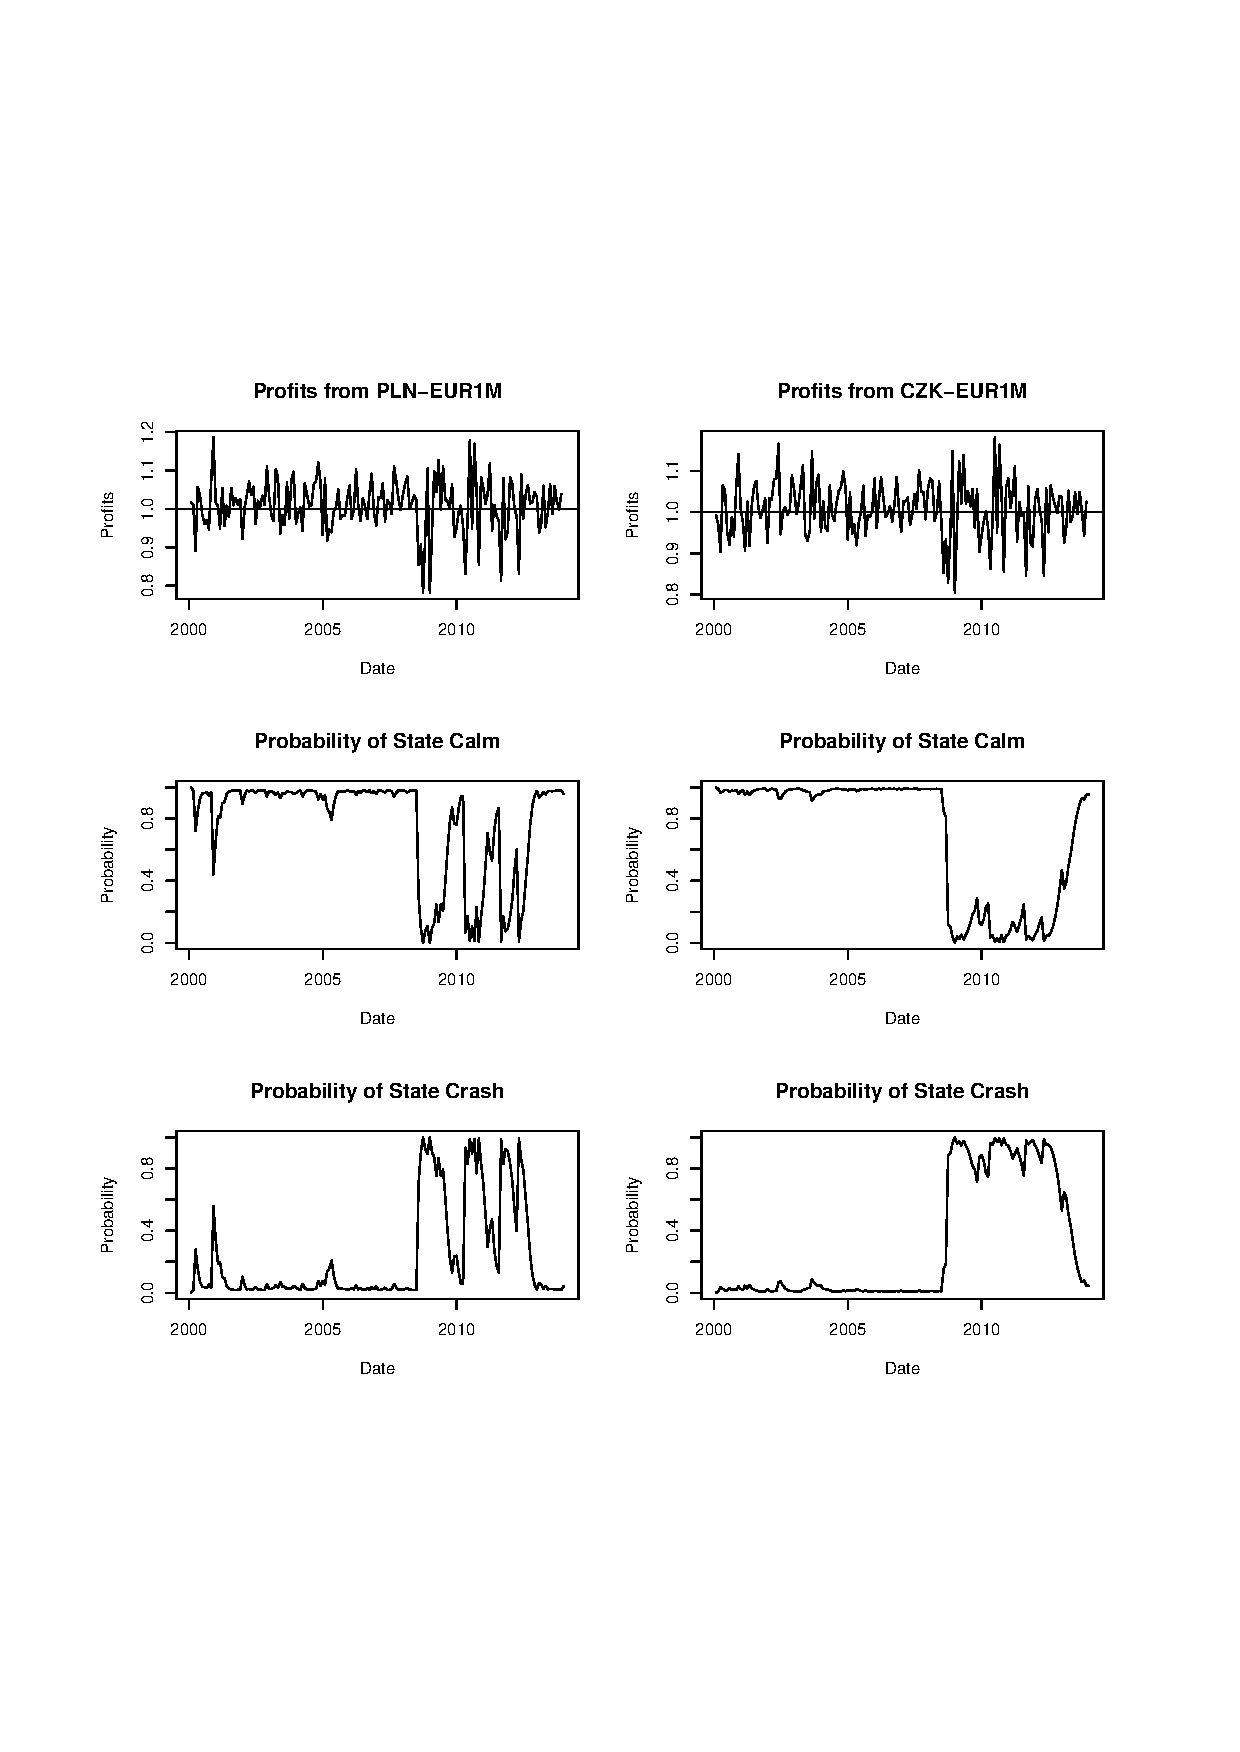
\includegraphics[scale = .75]{../Figures/2RegProb/PLNCZKEUR.pdf}
\end{figure}

\begin{figure}[h!]
\centering
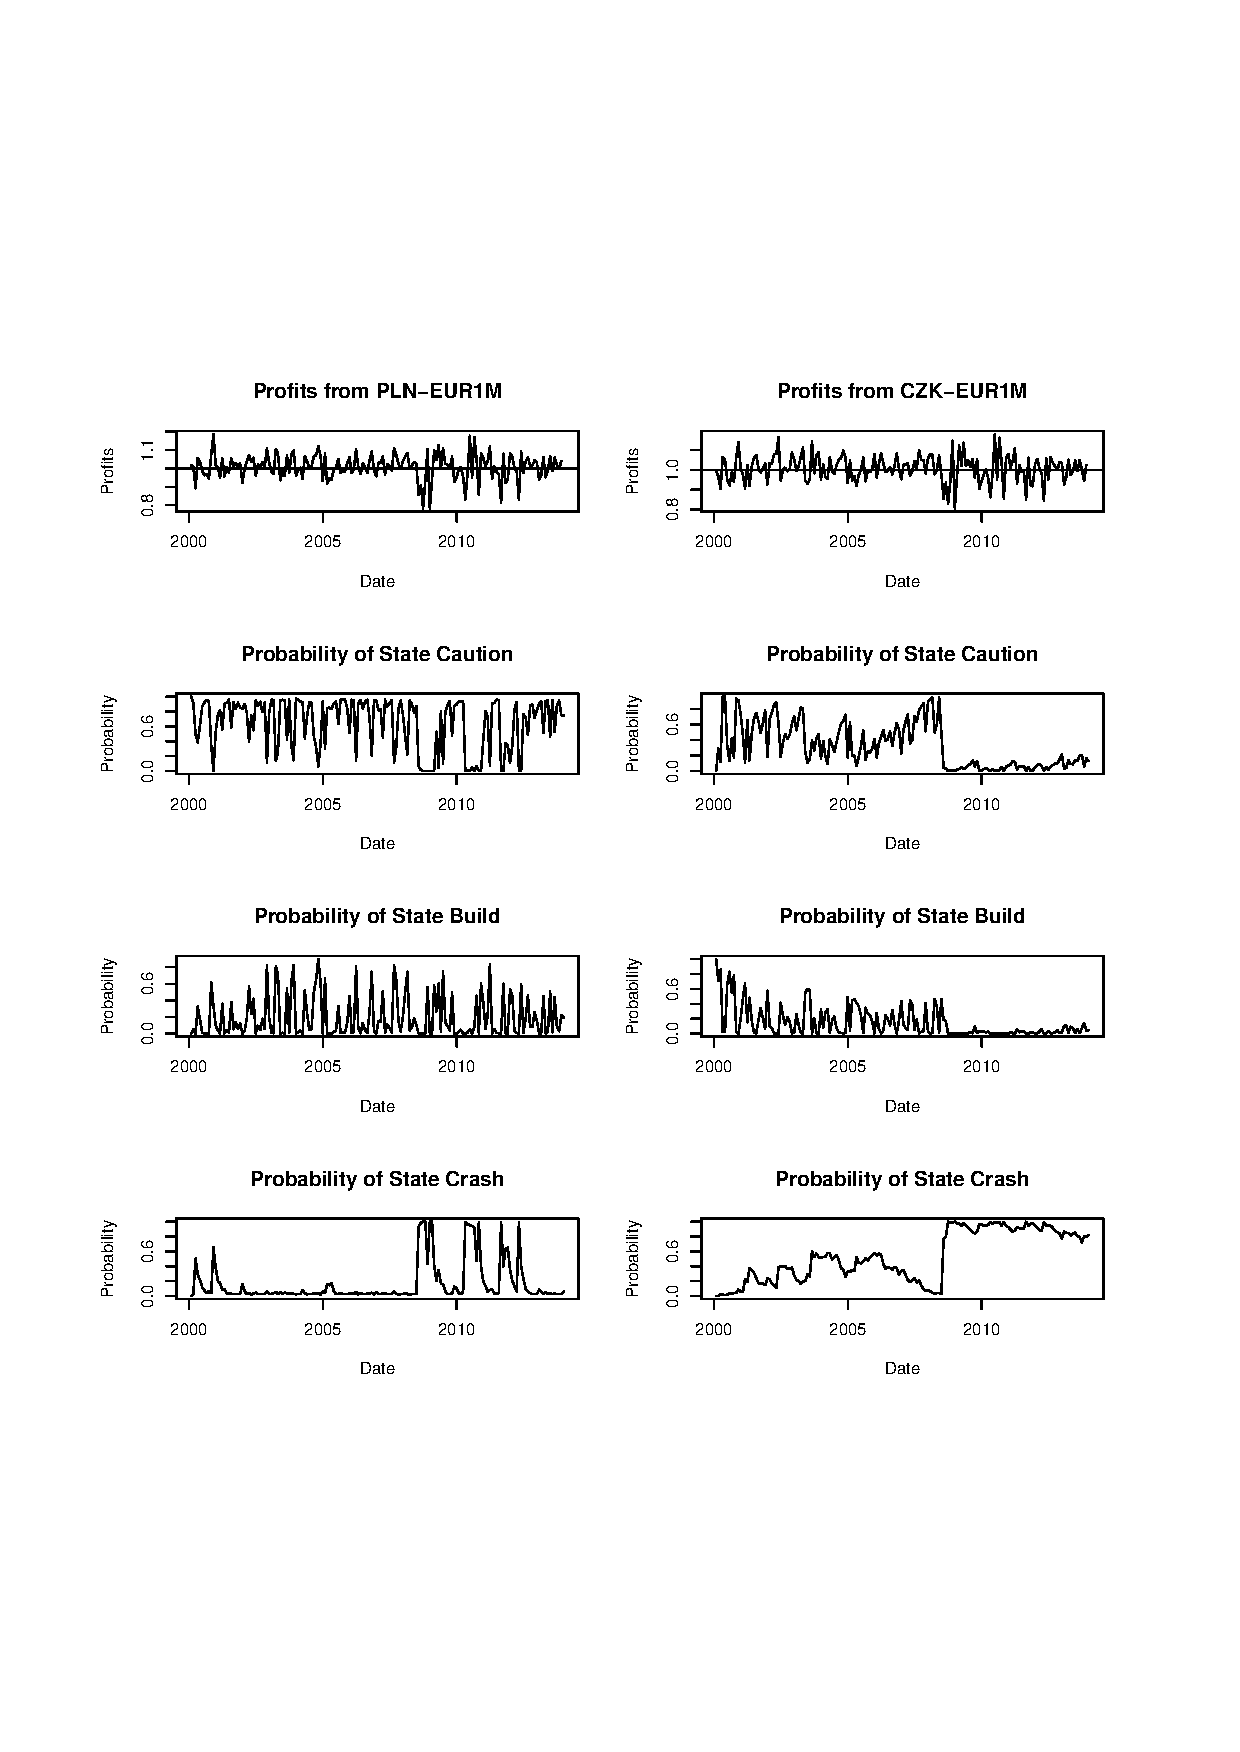
\includegraphics[scale = .80]{../Figures/3RegProb/PLNCZKEUR.pdf}
\end{figure}

\begin{figure}[h!]
\centering
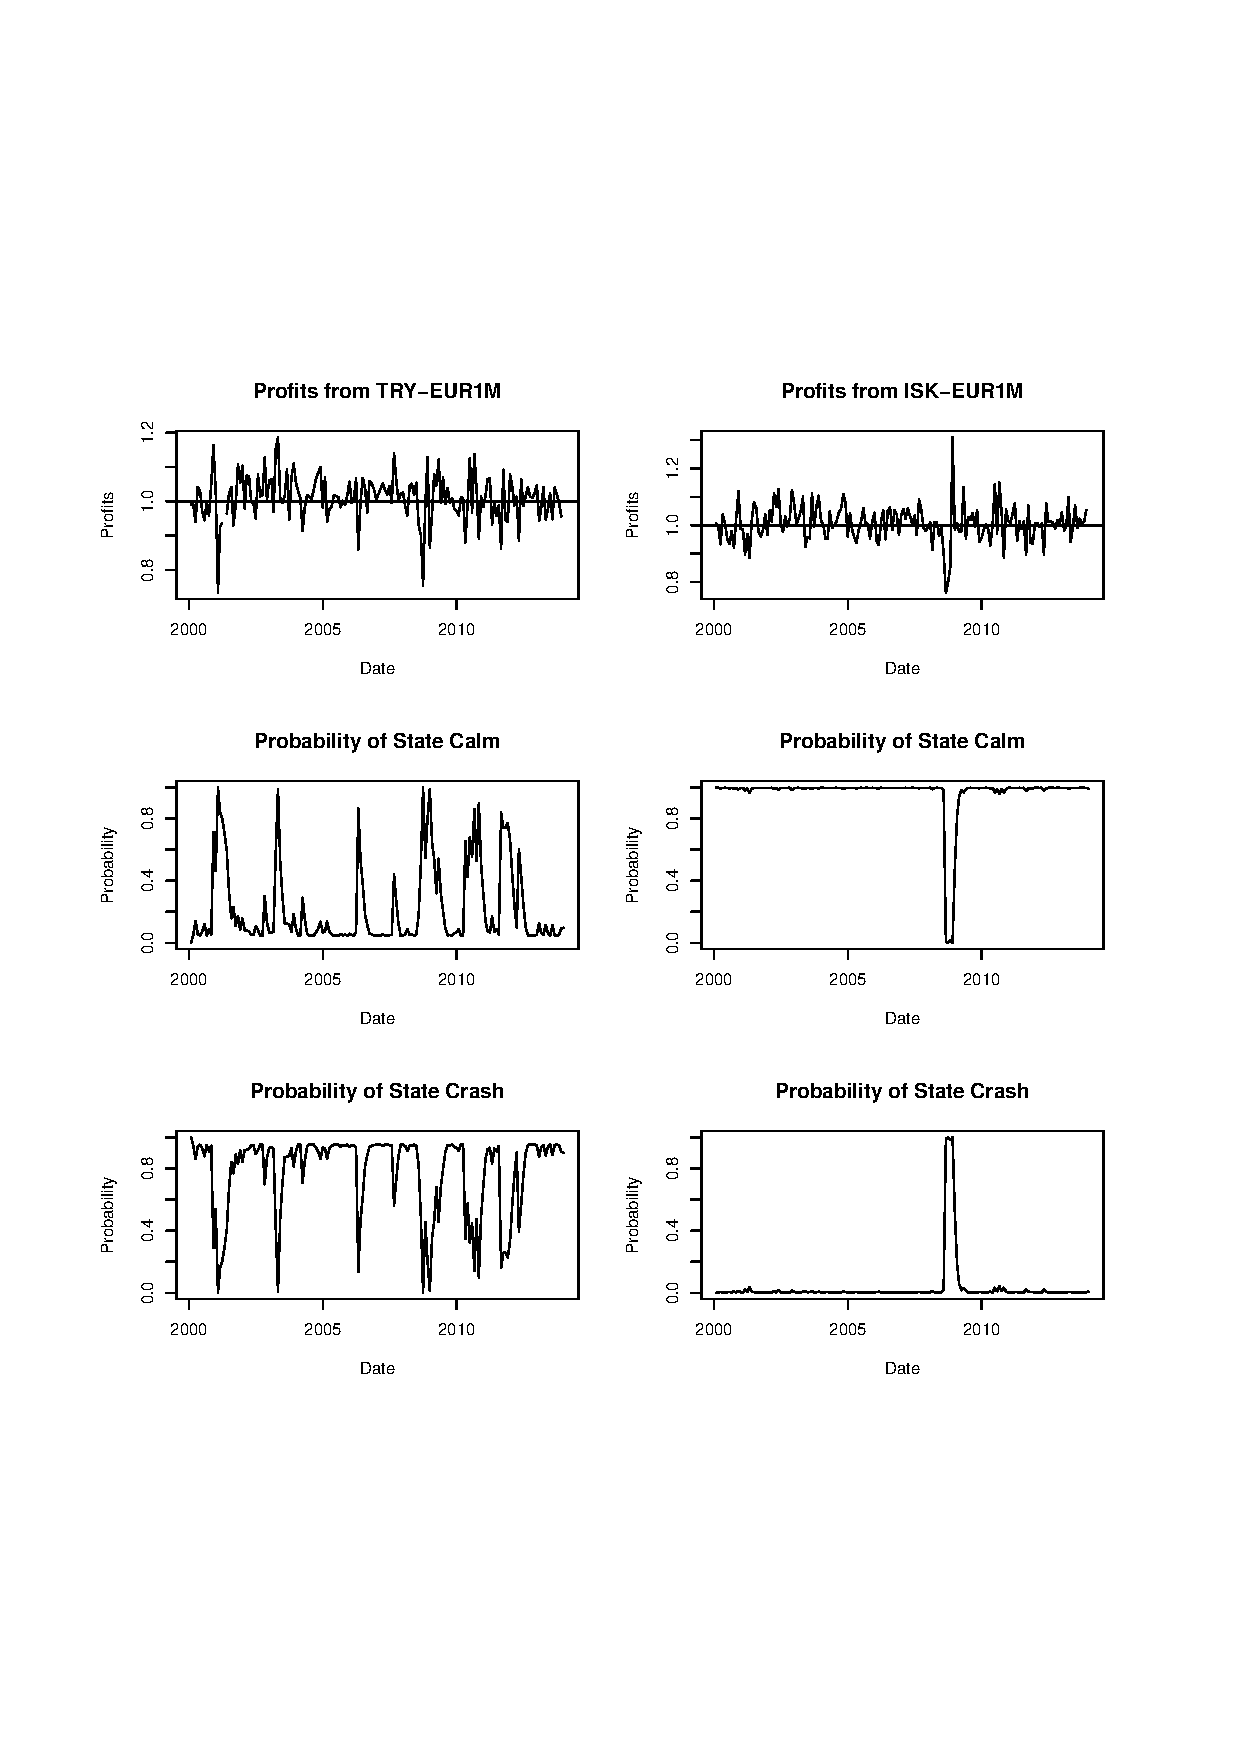
\includegraphics[scale = .80]{../Figures/2RegProb/ISKTRYEUR.pdf}
\end{figure}

\begin{figure}[h!]
\centering
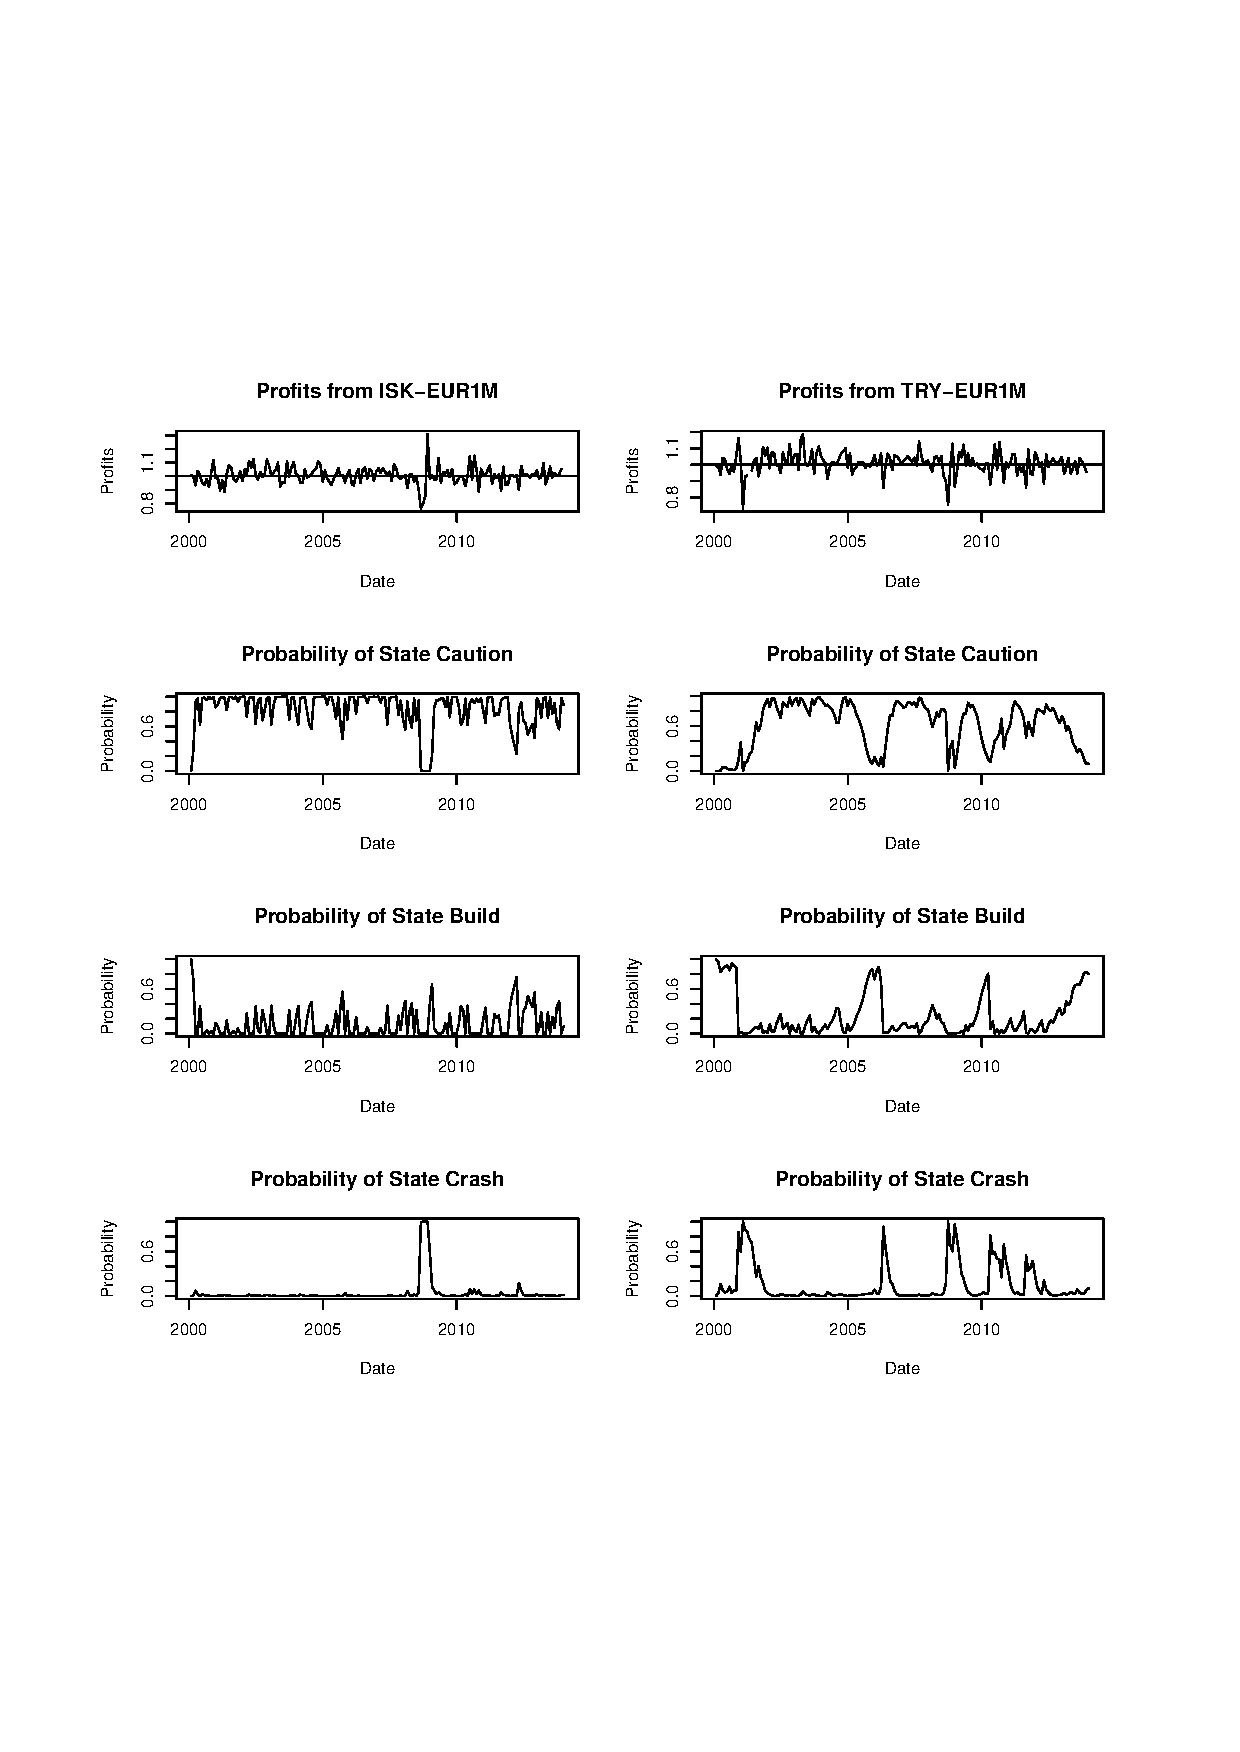
\includegraphics[scale = .80]{../Figures/3RegProb/ISKTRYEUR.pdf}
\end{figure}

\begin{figure}[h!]
\centering
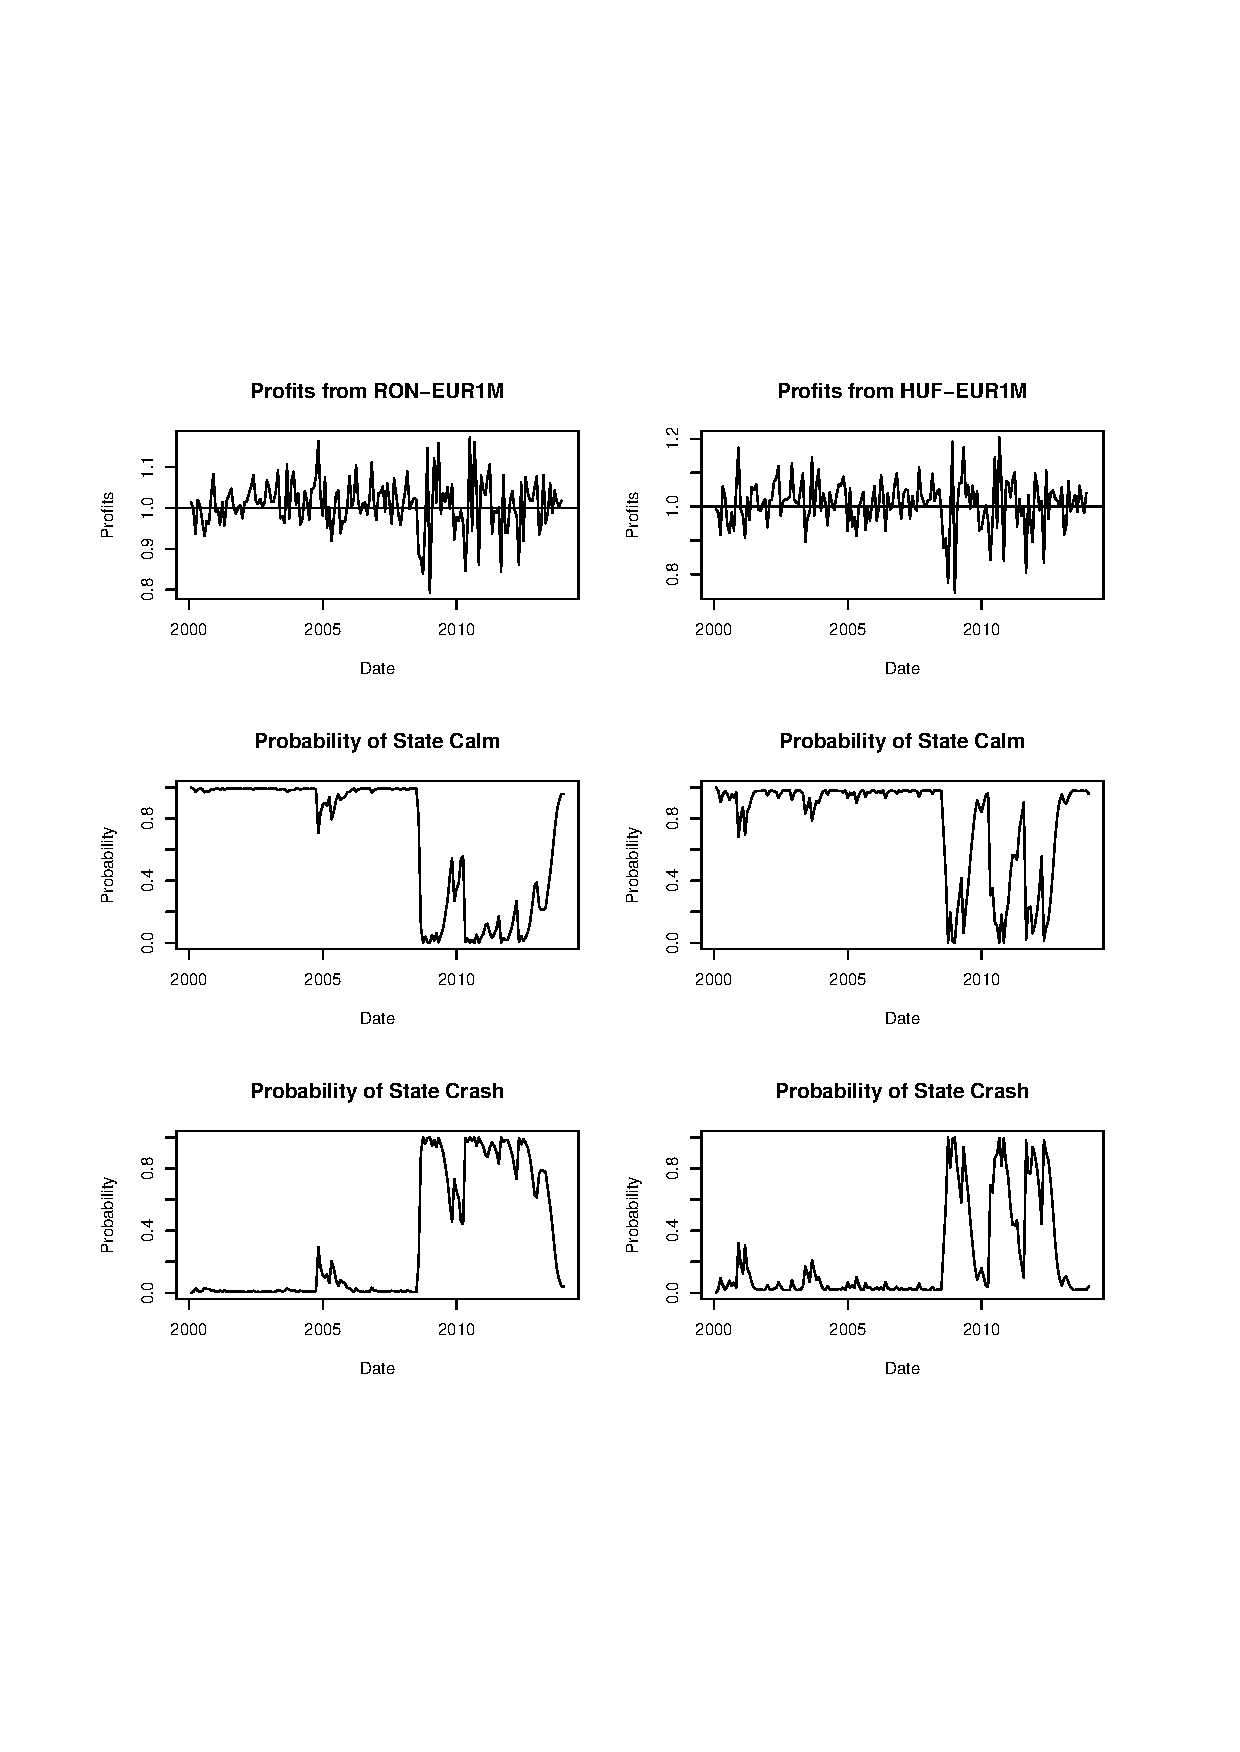
\includegraphics[scale = .80]{../Figures/2RegProb/RONHUFEUR.pdf}
\end{figure}

\begin{figure}[h!]
\centering
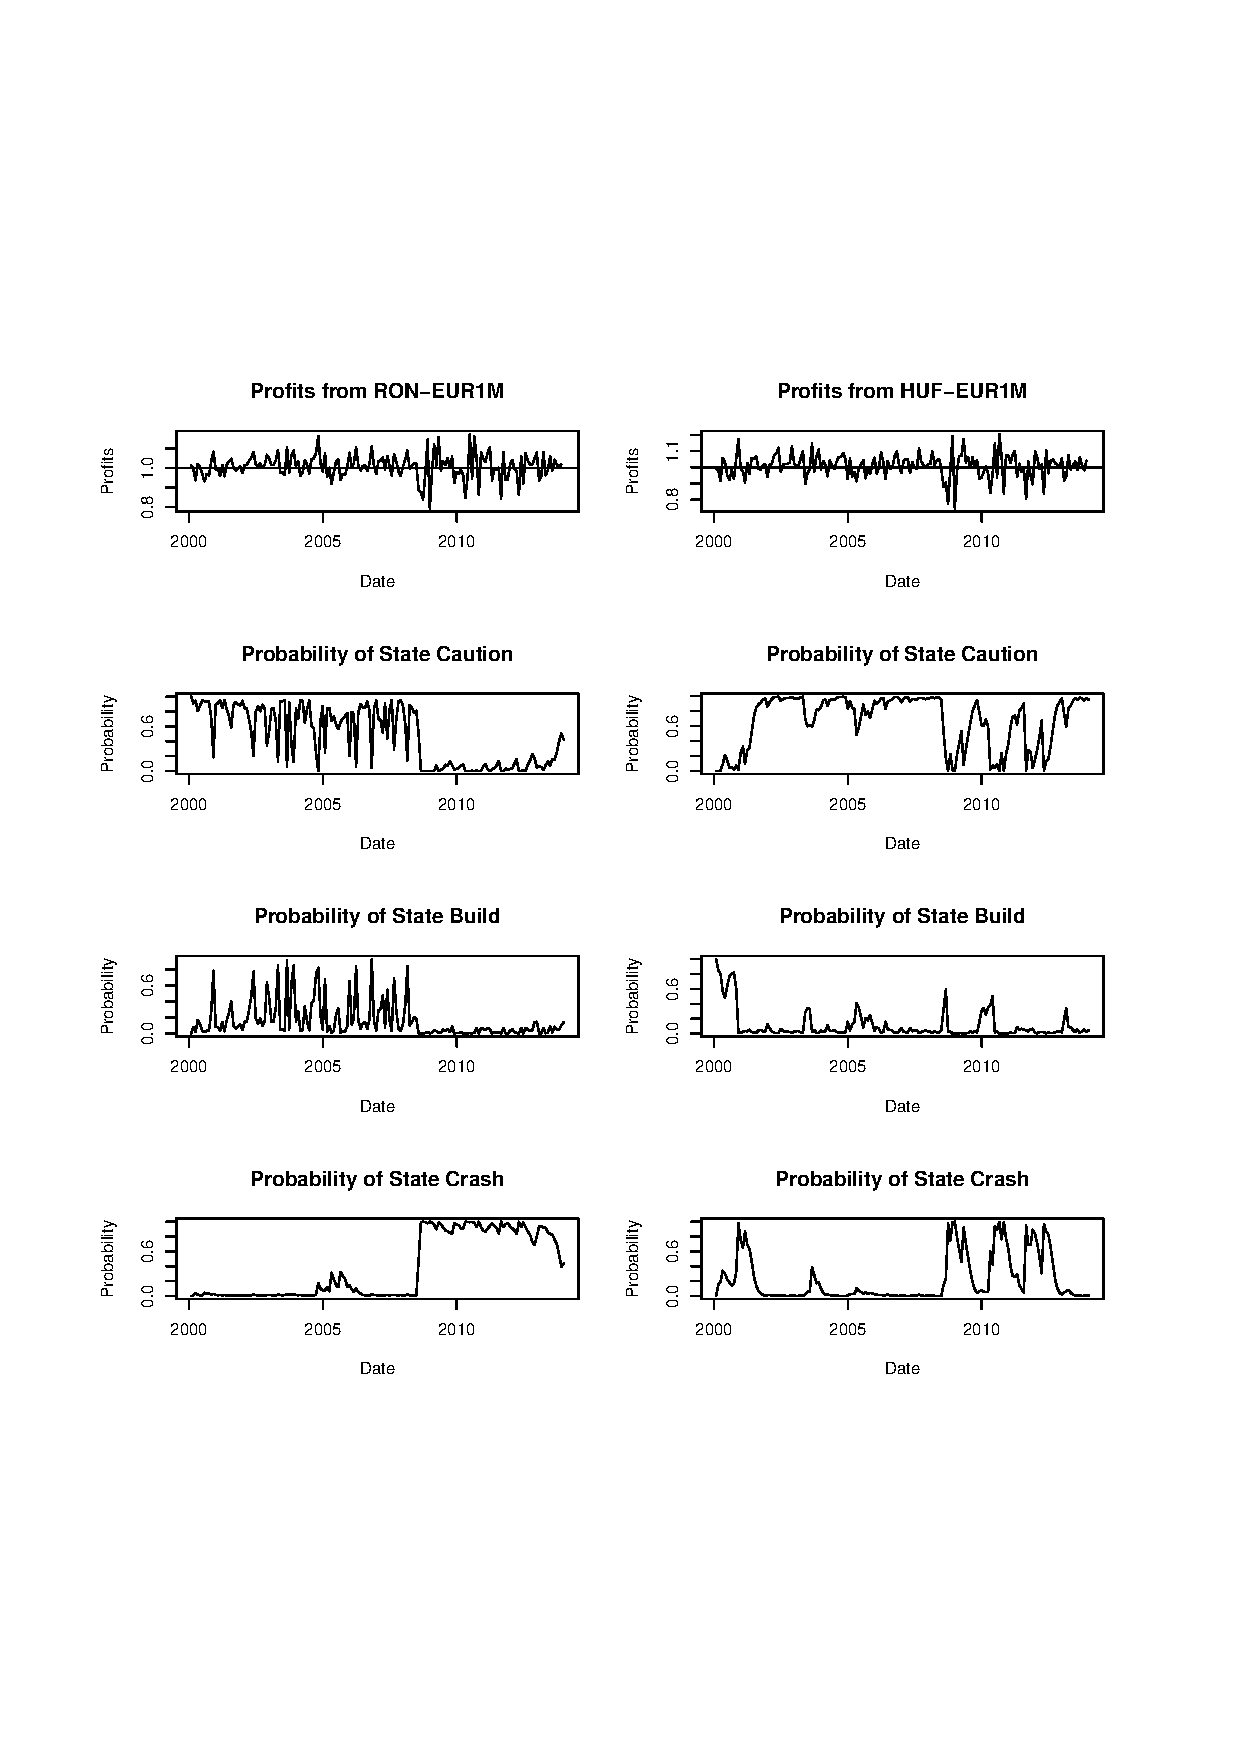
\includegraphics[scale = .80]{../Figures/3RegProb/RONHUFEUR.pdf}
\end{figure}

\begin{figure}[h!]
\centering
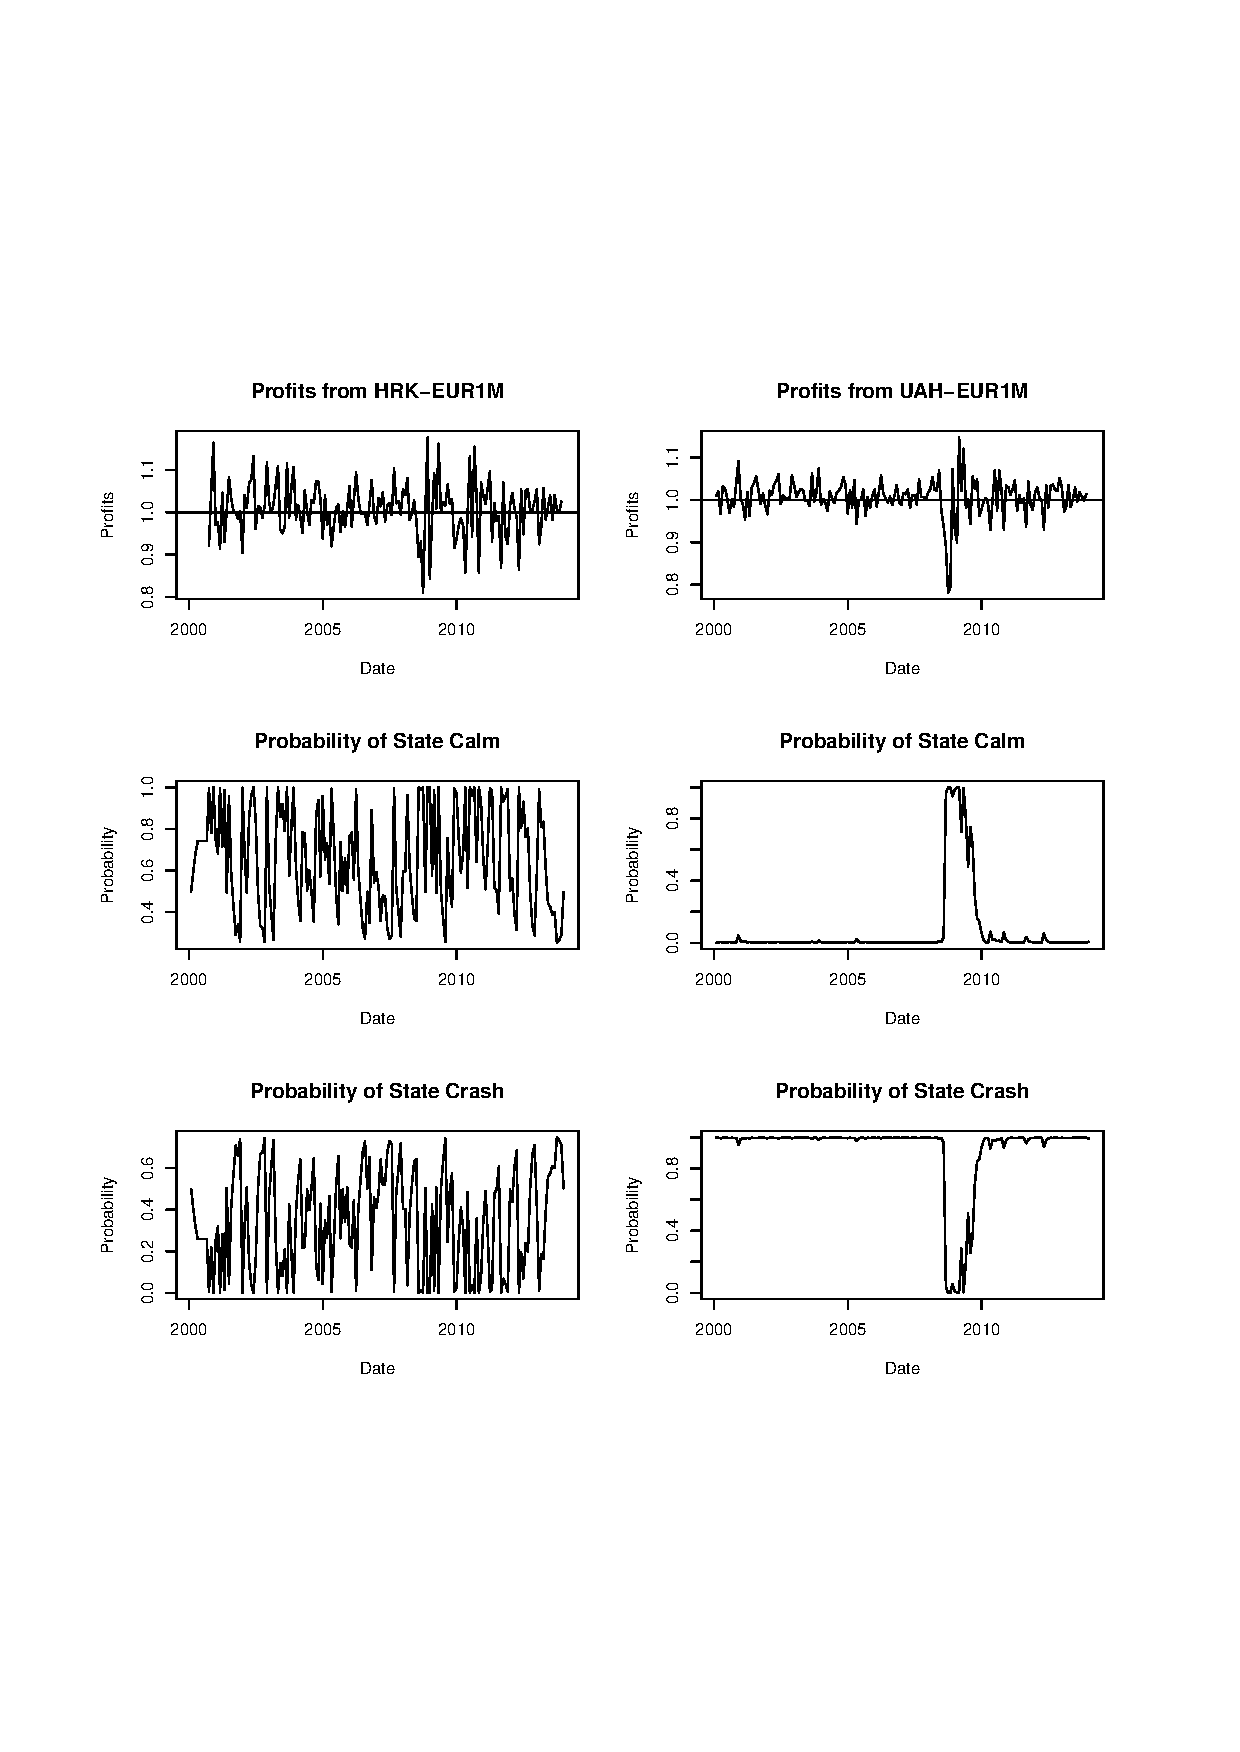
\includegraphics[scale = .80]{../Figures/2RegProb/HRKUAHEUR.pdf}
\end{figure}

\begin{figure}[h!]
\centering
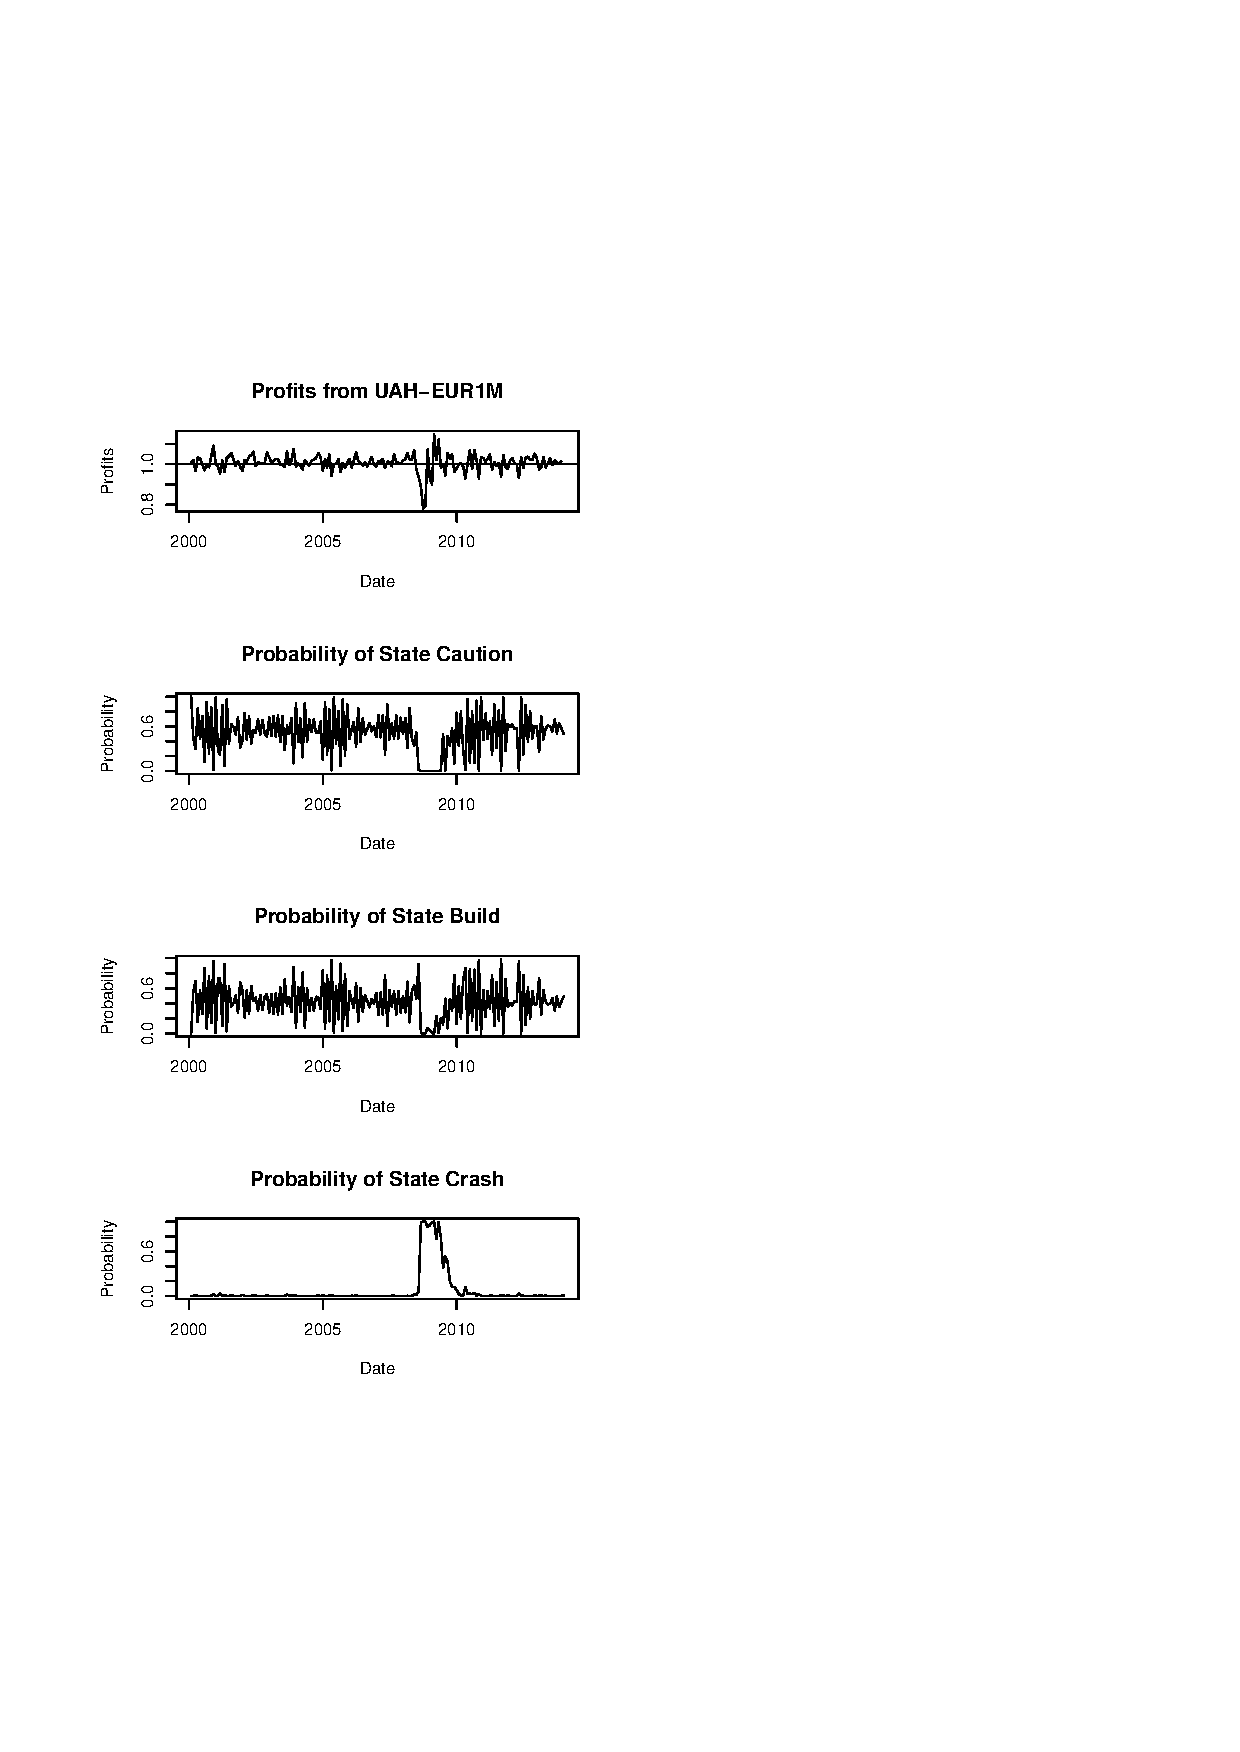
\includegraphics[scale = .80]{../Figures/3RegProb/HRKUAHEUR.pdf}
\end{figure}

This suggests that the crash is pretty rare as are the periods of caution. 


This suggests that the crash is pretty rare as are the periods of caution. 



\begin{figure}[h!]
\centering
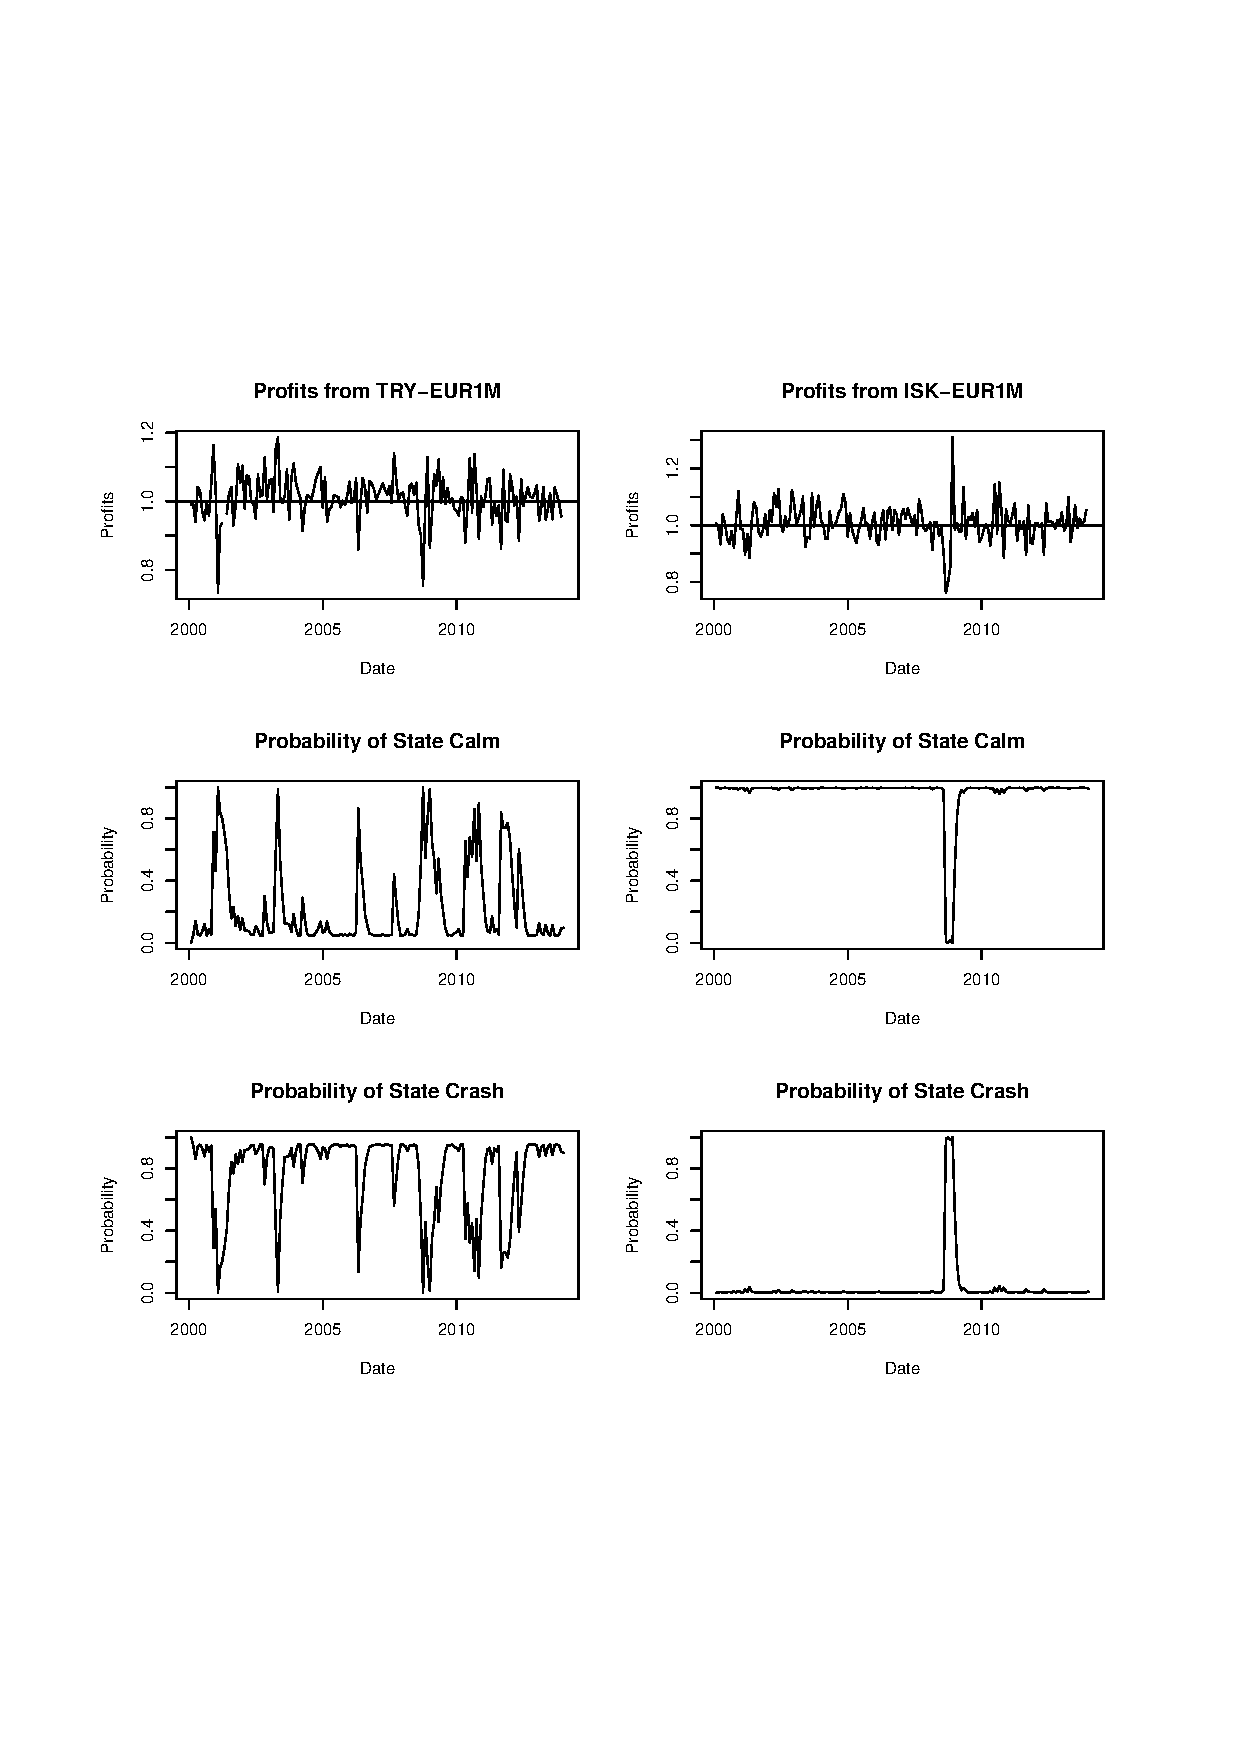
\includegraphics[scale = .80]{../Figures/2RegProb/ISKTRYEUR.pdf}
\end{figure}
% There are some issues with the creation of this figure.  It works in la tex stand alone.  


\section{Conclusions}
There are a number of ways that these methods can be used. 

Does the system evolve according to the three-regimes?  What are the characteristics of those cases where three-regime system does not work?  

What are the dates of the crash?  Which data are very similar for different currencies and which are unique.  What are the characteristics of the common crashes?  Do they relate to monetary, liquidity or risk shocks?  What are the characteristics of the unique crashes?  Do they relate to the international shocks.  It is more likely that they are domestic. 

What are the extensions and next steps.  A sophisticated model could allow the parameters to change over time.  One example would be to increase the probability of a crash as the time in the building phase or to relate the probability of a crash to some outside variables. 

Have a look at the probabilities of a crash that existed on particular days (ahead of the Lehman crisis)?  Do these probabilities say something about potential vuilnerability.  This can go into the table that assesses the reliability of the models.  What is the relatioknship between the vulnerability at the point of financial crisis and the subsequent ecomnomic outcome?  What is the relationship between the vulernablity and other characteristics? 

Other variables can be added to the model.  There are the carry-trade crash variables.  Could also add stock index. Will this add anything?  Could add a variable of EU political uncertainty. 


---------------------
From \citet{rabiner1989tutorial}.  There are three problems:
\begin{itemize}
\item Given the observations, what is the probability of observing sequence given the model? 
\item What is the sequence of unobserved states that best describes the observed.  There is an attempt to find the optimal sequence.  A comparison of problem one can be used. 
\item Optimise the parameters to best descibe the observed sequence. 
\end{itemize}

Use problem three to optimise the parameters of the observables given the latent states; use problem two to uncover the unobserved states; use problem one to calculate the probabilty of the observation given the paramers. 

Steps. 
\begin{itemize}
\item Maximise $P(O \lambda)$, where $\lambda = (\pi, A, B)$.  The probability of observing seqence O for a given set of parameters.  The easiest way of doing this is to calculate the probability for each of the possible state sequences.  Consider one such sequence, $Q = q_1 q_2 \dots q_T$, the probability of the observed sequence for the state sequence Q is $P(O|Q \lambda) = \prod_{t = 1}^T P(O_t|q_t, \lambda)$.  If the observations are independent, this probability $P(O|Q \lambda)$ is equal to the probabilty of observing the outcome given the state, $b_{q_1}(O_1)\dot b_{q_2} (O_2) \dots b_{q_T}(O_T)$.  At each step, the forward variable $\alpha_t(i) = P(O_1 O_2 \dots O_t, q_t = S_i|\lambda)$ is calculated as the product of the sum of all the probability of each state for the previous period and the probability of transition from each of those states to the current as well as the product of being in this state given the observable. $\alpha_t(i)$ is the joint probability that observation is seen and state is achieved. 
\item Optimise the hidden state sequence given the parameters 
\item From a number of $\lambda$ models, chose the most optimal. 
\end{itemize}


%\item There are probabilities for the system being in a crash situtation.  It is possible to look at the relatioship between this probability and other variables to assess the way that other factors can affect the fragility of the regime.  Examples that may be of use include the level of internatioal risk aversion (say the VIX index), the stacne of US monetary policy (either the level of rates of the expansionary nature of the policy if measured in other ways).  Confidnece in the banking system of financial centers.  For example, the spread between risk-free and banking assets in Us or Euro area. This can help to develop some understanding of the causes of international financial crises. 
%\item It should be possible to determine the current level of financial fragility.  The probability that the regime is in a state of crash could be used to compare countries and to assess the evolution of financial risk over time.  
%\item THere can be a comparison of different cultures and customs. Where are the similarities and where are the differences?  Different institutions may have different effects. Exchange rate regimes, level of financial development. 


%\href{http://a-little-book-of-r-for-bioinformatics.readthedocs.org/en/latest/src/chapter10.html}{Chapter 10 Biometric Text on HMM}
%has an excellent overview of markov HMM and the R code necessary. One component of this that could be of interest is the assertion in on-line bimetrixs text that it is a problem to find the underlying state that produced the DNA outcome.  The equivalent of this for the crash model is to find the underlying Minsky state that produced the market activity.

% latex table generated in R 3.0.2 by xtable 1.7-1 package
% Mon Aug 18 16:10:46 2014
\begin{landscape}
\begin{table}[ht]
\centering
\begin{tabular}{l|rrrrrrrrrrrr}
  \hline
 & AIC1 & BIC1 & AIC2 & BIC2 & LR21 & LR21p & AIC3 & BIC3 & LR31 & LR31p & LR32 & LR32p \\ 
  \hline
HUF & -404.69 & -398.46 & -419.50 & -391.44 & 28.81 & 0.0002 & -408.43 & -346.07 & 39.74 & 0.0023 & 10.94 & 0.4487 \\ 
  PLN & -423.98 & -417.74 & -438.93 & -410.87 & 28.95 & 0.0001 & -424.77 & -362.41 & 36.79 & 0.0001 & 7.84 & 0.7278 \\ 
  CZK & -427.23 & -421.00 & -430.52 & -402.46 & 17.29 & 0.0156 & -426.74 & -364.38 & 35.51 & 0.0002 & 18.22 & 0.0766 \\ 
  RON & -456.02 & -449.78 & -478.07 & -450.01 & 36.05 & 0.0000 & -473.04 & -410.68 & 53.02 & 0.0000 & 16.97 & 0.1087 \\ 
  RUB & -456.02 & -449.78 & -566.68 & -538.62 & 124.67 & 0.0000 & -556.35 & -493.99 & 136.33 & 0.0000 & 11.66 & 0.3894 \\ 
  BGN & -451.98 & -445.75 & -459.55 & -431.49 & 21.56 & 0.0030 & -556.35 & -493.99 & 140.37 & 0.0000 & 118.80 & 0.0000 \\ 
  NOK & -453.92 & -447.69 & -445.70 & -417.64 & 5.78 & 0.5656 & -556.35 & -493.99 & 138.42 & 0.0000 & 132.64 & 0.0000 \\ 
  ISK & -439.36 & -433.12 & -463.57 & -435.51 & 38.22 & 0.0000 & -447.99 & -385.63 & 44.63 & 0.0000 & 6.42 & 0.8441 \\ 
  UAH & -572.87 & -566.64 & -647.67 & -619.61 & 88.80 & 0.0000 & -447.99 & -385.63 & -88.88 & 1.0000 & -177.68 & 1.0000 \\ 
  HRK & -431.55 & -425.41 & -439.42 & -411.80 & 21.87 & 0.0027 & -408.43 & -346.07 & 12.89 & 0.7983 & -8.99 & 1.0000 \\ 
  TRY & -431.05 & -424.83 & -439.26 & -411.25 & 22.20 & 0.0023 & -434.70 & -372.46 & 39.65 & 0.0023 & 17.45 & 0.0954 \\ 
   \hline
\end{tabular}
\caption{Comparison of models table} 
\label{tabref:comptab}
\end{table}
\end{landscape}

\begin{landscape}
% latex table generated in R 3.0.2 by xtable 1.7-1 package
% Wed Aug 20 15:33:19 2014
\begin{table}[ht]
\centering
\begin{tabular}{rrrrrrrrrr}
  \hline
 & AIC1 & ACI1a & AIC2a & LR21 & LR21p & LR31 & LR31p & Conf1 & Conf2 \\ 
  \hline
HUF & -404.69 & -402.76 & -414.07 & 0.07 & 0.7915 & 23.40 & 0.0015 & -0.0059 & 0.0045 \\ 
  PLN & -423.98 & -422.01 & -437.68 & 0.03 & 0.8572 & 27.70 & 0.0002 & -0.0053 & 0.0045 \\ 
  CZK & -427.23 & -425.29 & -424.90 & 0.06 & 0.8139 & 11.70 & 0.1121 & -0.0054 & 0.0043 \\ 
  RON & -456.02 & -454.03 & -473.35 & 0.01 & 0.9136 & 31.30 & 0.0001 & -0.0047 & 0.0042 \\ 
  RUB & -523.18 & -521.22 & -567.38 & 0.04 & 0.8365 & 58.20 & 0.0000 & -0.0040 & 0.0033 \\ 
  BGN & -451.98 & -449.99 & -451.72 & 0.00 & 0.9603 & 13.70 & 0.0561 & -0.0044 & 0.0046 \\ 
  NOK & -453.92 & -452.08 & -446.57 & 0.16 & 0.6911 & 6.60 & 0.4667 & -0.0054 & 0.0036 \\ 
  ISK & -439.36 & -437.44 & -461.94 & 0.08 & 0.7798 & 36.60 & 0.0000 & -0.0053 & 0.0040 \\ 
  UAH & -572.87 & -571.23 & -642.78 & 0.35 & 0.5517 & 83.90 & 0.0000 & -0.0041 & 0.0022 \\ 
  HRK & -431.55 & -429.64 & -430.07 & 0.09 & 0.7609 & 12.50 & 0.0847 & -0.0053 & 0.0039 \\ 
  TRY & -431.05 & -429.47 & -440.94 & 0.42 & 0.5166 & 23.90 & 0.0012 & -0.0063 & 0.0032 \\ 
   \hline
\end{tabular}
\caption{US rate model table} 
\label{tabref:comptab}
\end{table}
\end{landscape}

This table shows the comparison of three models.  The first is the simple regression of the carry-trade profit on the constant, the second is the carry trade profit on US interest rate and the third is the carry trade profit on US interest rate with two-regimes.  
\begin{landscape}
% latex table generated in R 3.0.2 by xtable 1.7-1 package
% Wed Aug 20 16:55:39 2014
\begin{table}[ht]
\centering
\begin{tabular}{rrrrrrrrrr}
  \hline
 & AIC1 & ACI2 & AIC3 & LR21 & LR21p & LR31 & LR31p & LR32 & LR32p \\ 
  \hline
HUF & -404.69 & -416.94 & -419.50 & 22.25 & 0.0005 & 28.80 & 0.0002 & 6.6000 & 0.0376 \\ 
  PLN & -423.98 & -437.62 & -434.65 & 23.65 & 0.0003 & 24.70 & 0.0009 & 1.0000 & 0.6000 \\ 
  CZK & -427.23 & -427.37 & -436.40 & 10.14 & 0.0714 & 23.20 & 0.0016 & 13.0000 & 0.0015 \\ 
  RON & -456.02 & -474.81 & -480.11 & 28.79 & 0.0000 & 38.10 & 0.0000 & 9.3000 & 0.0096 \\ 
  RUB & -523.18 & -567.77 & -571.33 & 54.59 & 0.0000 & 62.20 & 0.0000 & 7.6000 & 0.0228 \\ 
  BGN & -451.98 & -454.32 & -470.22 & 12.34 & 0.0305 & 32.20 & 0.0000 & 19.9000 & 0.0000 \\ 
  NOK & -453.92 & -449.12 & -457.62 & 5.20 & 0.3922 & 17.70 & 0.0134 & 12.5000 & 0.0019 \\ 
  ISK & -439.36 & -464.24 & -463.07 & 34.88 & 0.0000 & 37.70 & 0.0000 & 2.8000 & 0.2430 \\ 
  UAH & -572.87 & -643.36 & -645.68 & 80.49 & 0.0000 & 86.80 & 0.0000 & 6.3000 & 0.0426 \\ 
  HRK & -572.87 & -433.37 & -448.83 & -129.51 & 1.0000 & -110.00 & 1.0000 & 19.5000 & 0.0001 \\ 
  TRY & -431.05 & -441.00 & -443.33 & 19.95 & 0.0013 & 26.30 & 0.0005 & 6.3000 & 0.0423 \\ 
   \hline\
\end{tabular}
\caption{US rate model table2} 
\label{tabref:comptab}
\end{table}
\end{landscape}


This table shows the resutls of three models.  THe first is the base model, the second is the base model with 2 states and the third is the base model and 2 states with the transition probabilities affected by the change in US interest rates. 
\bibliography{myrefsRS}



\end{document}